%\documentclass{article}
%\usepackage[utf8]{inputenc}
%\usepackage{graphicx}
%\usepackage[main=greek,english]{babel}
%\newcommand\tab[1][1cm]{\hspace*{#1}}
%\newcommand \en {\selectlanguage{english}}
%\newcommand \gr {\selectlanguage{greek}}

%\begin{document}
%\gr
 
 \subsection{\en Fantasia Database \gr}
  Σε αυτές τις περιπτώσεις ο αλγόριθμος δεν είναι ιδιαίτερα εύστοχος. Η κατάσταση αυτή οφείλεται στο γεγονός ότι το σήμα αν και δεν είναι απόλυτα σταθερό, επειδή αποτελεί φυσιολογική καρδιακή δραστηριότητα, δεν αποκλίνει ιδιαίτερα ούτε διαθέτει έντονες αυξομειώσεις. Όταν, όμως, εμφανίζονται συγκεκριμένα απομονωμένα \en spikes, \gr εντοπίζονται άμεσα από τον αλγόριθμο και ταυτίζονται ως αφύσικες καρδιακές. Ως γενική εικόνα ο αλγόριθμος εδώ φαίνεται να μη διαθέτει την απαραίτητη ευστοχία. Για αυτό το λόγο, εφαρμόστηκαν τεχνητές αρρυθμίες και έκτοπες συστολές, όμοιες με αυτές της προπτυχιακής εργασίας με τίτλο "Εκτίμηση ιδιοτήτων της εντροπίας φυσαλίδων". Οι κατηγορίες των πειραμάτων ήταν οι:
  \begin{itemize}
      \item Μηδενισμός συνεχόμενων \en RR \gr διαστημάτων μέσα στο καρδιογράφημα (απώλεια συνεχόμενων παλμών, ύπαρξη συνεχόμενων \en skipped beats \gr).
      \item Πολλαπλασιασμός συνεχόμενων \en RR \gr διαστημάτων κατά κάποιο ακέραιο αριθμό. Ο ακέραιος αριθμός ήταν το 3.
      \item \en A B+C \gr: Ενσωμάτωση δύο διαστημάτων σε ένα μεγαλύτερης διάρκειας. Αυτό καταδεικνύει την καθυστέρηση κάποιου παλμού, δημιουργώντας ένα πλατύτερο \en RR \gr διάστημα.
      \item \en A x B-x C \gr: Σε αυτή την περίπτωση διαπιστώνεται η παρεμβολή ενός διαστήματος \en x \gr, δηλαδή ενός επιπλέον παλμού και ο παλμός Β δε μετακινείται (συμβαίνει δηλαδή κανονικά). Στη συνέχεια οι παλμοί πραγματοποιούνται φυσιολογικά.
      \item \en A x B C \gr: Αντίθετα με πριν, ο Β παλμός μετακινείται (συμβαίνει δηλαδή σε διαφορετική χρονική στιγμή). Το ίδιο συμβαίνει και με όλους τους επόμενους παλμούς, προκαλόντας μια ολίσθηση.
      \item \en A x C \gr: Δεν υπάρχει κάποιος επιπρόσθετος παλμός. Παρουσιάζεται μια διαταραχή στο Β παλμό, που μπορεί να σημαίνει τη μετακίνησή του προς τα δεξιά ή τα αριστερά (να προηγηθεί ή να καθυστερήσει χρονικά). Αυτό μπορεί να συμβεί λόγω σφάλματος του αλγορίθμου εντοπισμού του \en QRS \gr συμπλέγματος, που μπορεί λόγω ύπαρξης θορύβου να εντοπίσει την κορυφή \en R \gr σε διαφορετικό σημείο. Επιπλέον, εκτός από την ύπαρξη θορύβου, μικρές μετατοπίσεις του Β μπορεί να οφείλονται και στη χαμηλή συχνότητα δειγματοληψίας του σήματος.
  \end{itemize}

Προς αποφυγή επαναλήψεων, μιας και τα αποτελέσματα για κάθε μετρική/ μέθοδο ήταν όμοια για κάθε τύπο πειράματος θα σχολιαστούν όλα στην ίδια παράγραφο. 
\par
Η αρχική εικόνα των καταγραφών ήταν η (Σχήμα 4.123):

\begin{figure}[h!]
    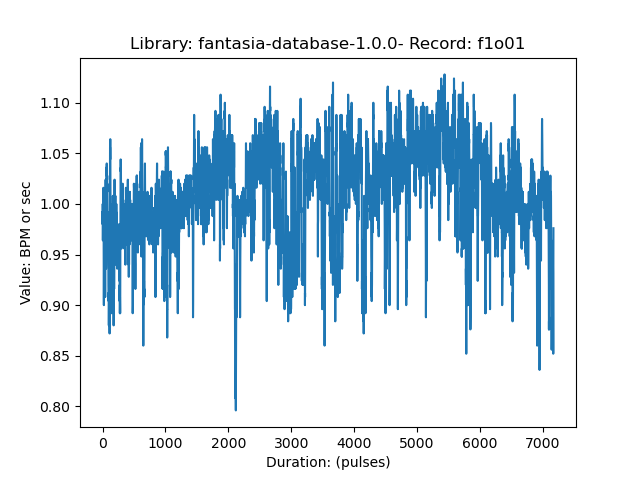
\includegraphics[width=.24\textwidth]{Fantasia/fantasia-database-1.0.0_f1o01.png}\hfill
    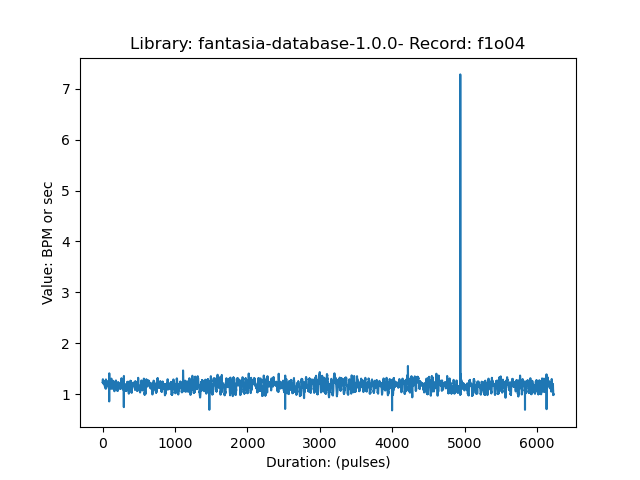
\includegraphics[width=.24\textwidth]{Fantasia/fantasia-database-1.0.0_f1o04.png}\hfill
    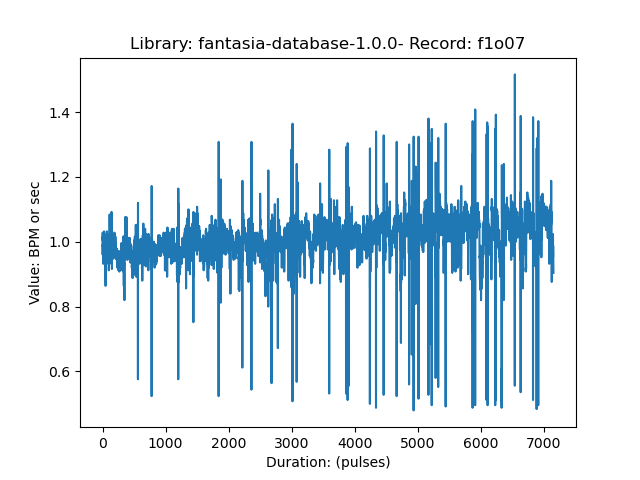
\includegraphics[width=.24\textwidth]{Fantasia/fantasia-database-1.0.0_f1o07.png}\hfill
    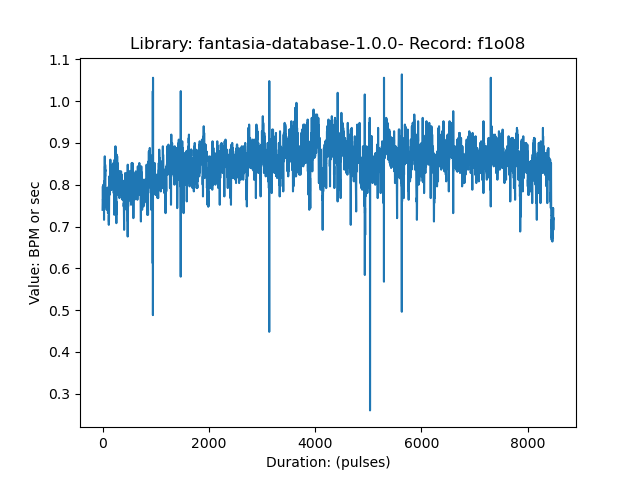
\includegraphics[width=.24\textwidth]{Fantasia/fantasia-database-1.0.0_f1o08.png}\hfill
   \\[\smallskipamount]
    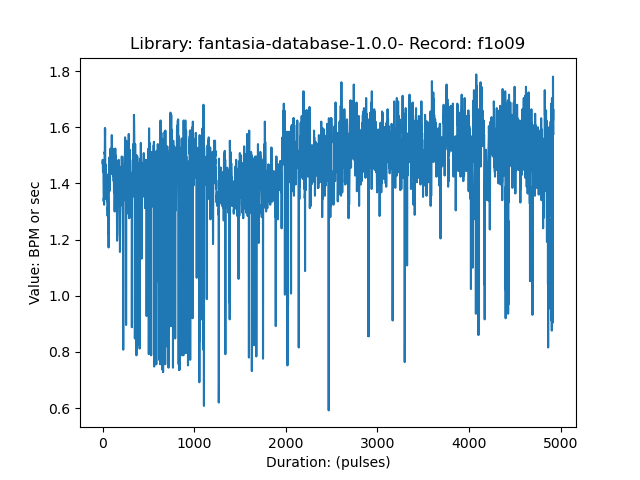
\includegraphics[width=.24\textwidth]{Fantasia/fantasia-database-1.0.0_f1o09.png}\hfill
    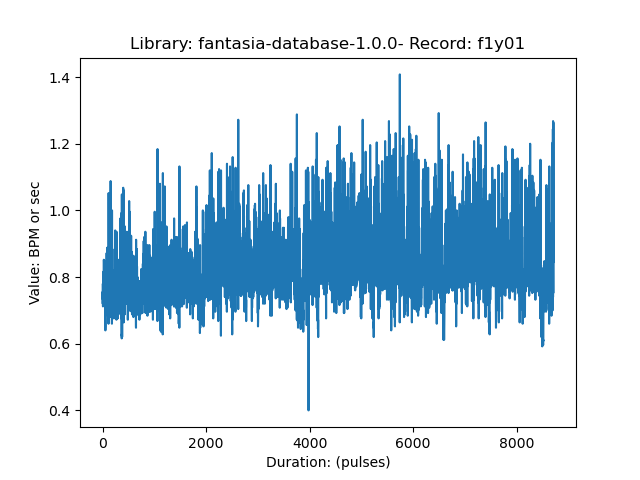
\includegraphics[width=.24\textwidth]{Fantasia/fantasia-database-1.0.0_f1y01.png}\hfill
    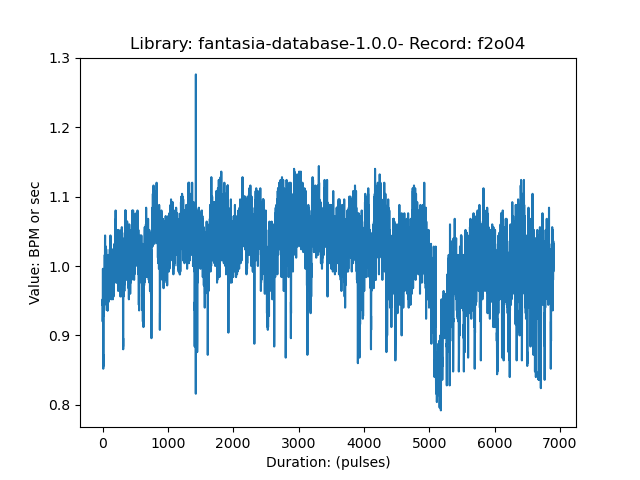
\includegraphics[width=.24\textwidth]{Fantasia/fantasia-database-1.0.0_f2o04.png}\hfill
    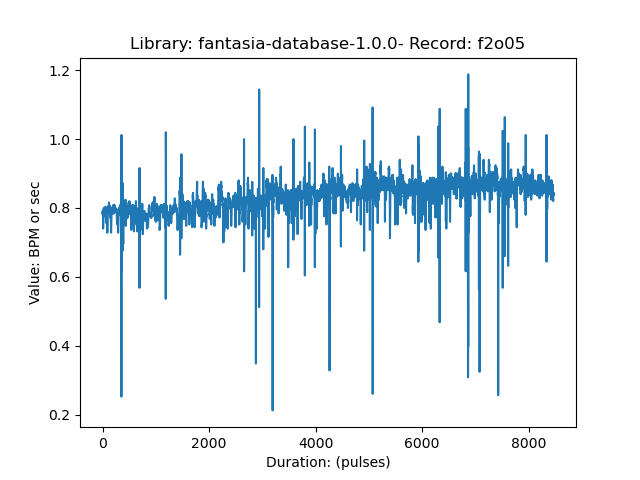
\includegraphics[width=.24\textwidth]{Fantasia/fantasia-database-1.0.0_f2o05.png}\hfill
    \\[\smallskipamount]
    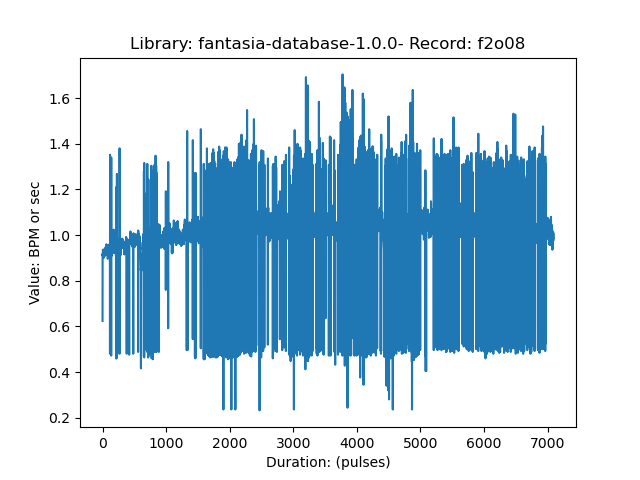
\includegraphics[width=.24\textwidth]{Fantasia/fantasia-database-1.0.0_f2o08.png}\hfill
    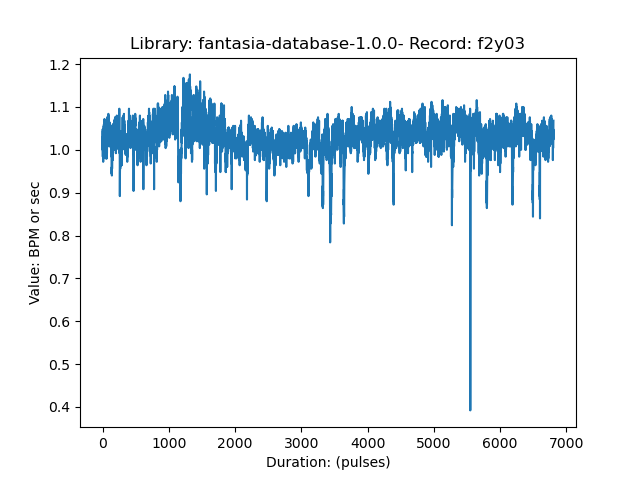
\includegraphics[width=.24\textwidth]{Fantasia/fantasia-database-1.0.0_f2y03.png}\hfill
    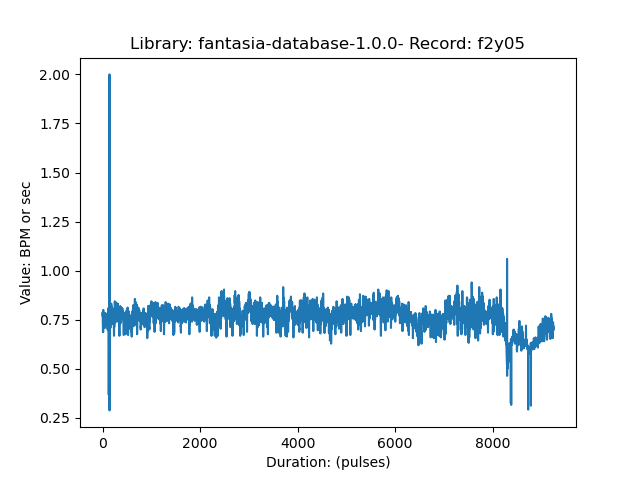
\includegraphics[width=.24\textwidth]{Fantasia/fantasia-database-1.0.0_f2y05.png}\hfill
    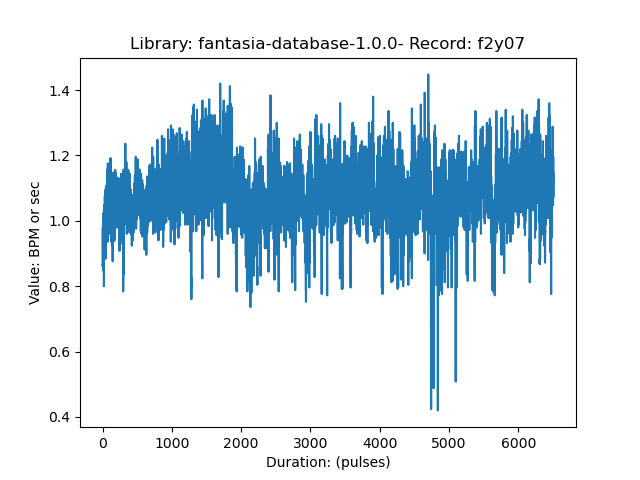
\includegraphics[width=.24\textwidth]{Fantasia/fantasia-database-1.0.0_f2y07.png}\hfill
    \caption{Συλλογή αποτελεσμάτων από τη βιβλιοθήκη \en Fantasia Database \gr (αρχικά δείγματα/καταγραφές)}
\end{figure}

\par
Μετά την εφαρμογή των διαφορετικών αρρυθμιών και έκτοπων παλμών στα σήματα, τα αποτελέσματα ήταν τα εξής:

\begin{itemize}
    \item \en ApEn: \gr Αυτή η βιβλιοθήκη φαίνεται να μην ευνοεί τις εκτιμήσεις της \en ApEn, \gr μιας και τα αποτελέσματά της είναι από τα πιο αδύναμα. Ο τρόπος με τον οποίο δημιουργήθηκαν τα πρόσθετα πειράματα τα κάνει να διακρίνονται πολύ εύκολα. Το γεγονός ότη η \en ApEn \gr αποτυγχάνει ενισχύει το σχόλιο πως δεν αποτελεί κατάλληλη μέθοδο για την εκτίμηση των περιοχών που ζητούνται. Οι εκτιμήσεις φαίνονται εδώ (Σχήμα 4.124) 

\begin{figure}[h!]
    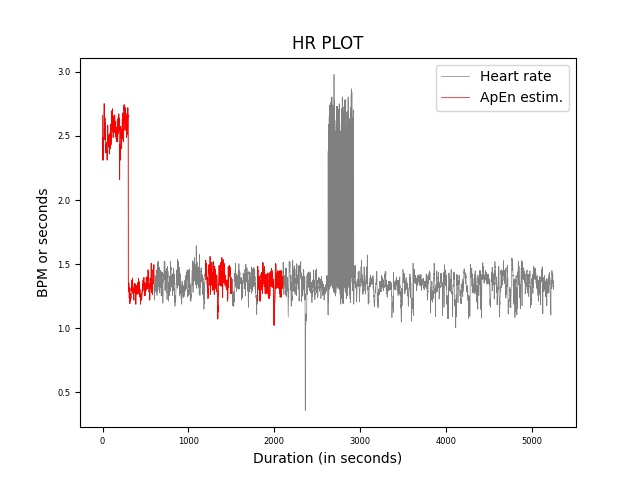
\includegraphics[width=.24\textwidth]{fantasia-Apen/1/fantasia-database-1.0.0_16_f2o06_300sec .jpeg}\hfill
    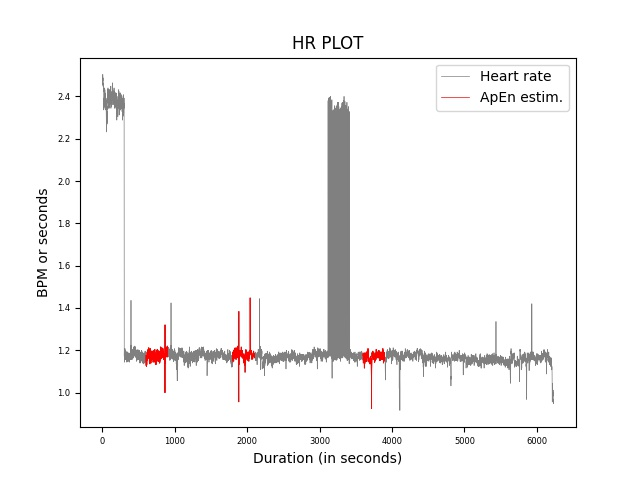
\includegraphics[width=.24\textwidth]{fantasia-Apen/1/fantasia-database-1.0.0_19_f1o06_300sec .jpeg}\hfill
    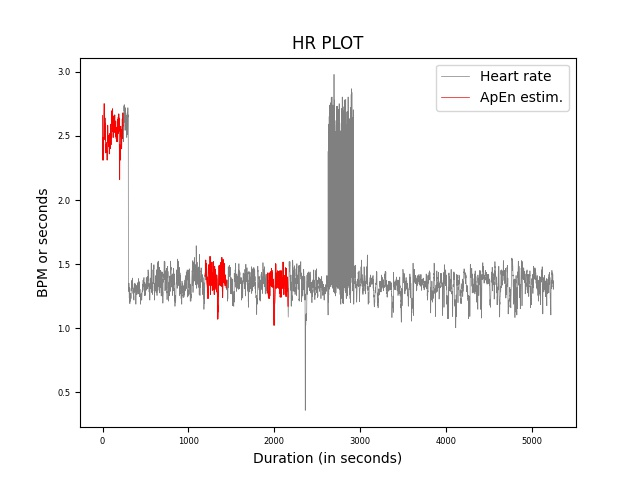
\includegraphics[width=.24\textwidth]{fantasia-Apen/1/fantasia-database-1.0.0_20_f2o06_240sec .jpeg}\hfill
    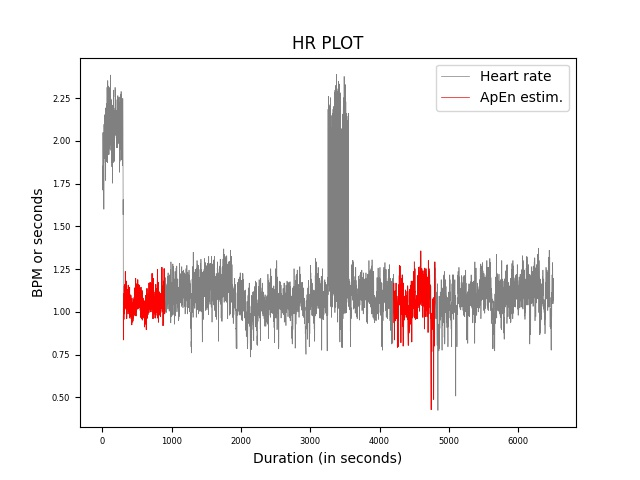
\includegraphics[width=.24\textwidth]{fantasia-Apen/1/fantasia-database-1.0.0_20_f2y07_300sec .jpeg}\hfill
   \\[\smallskipamount]
    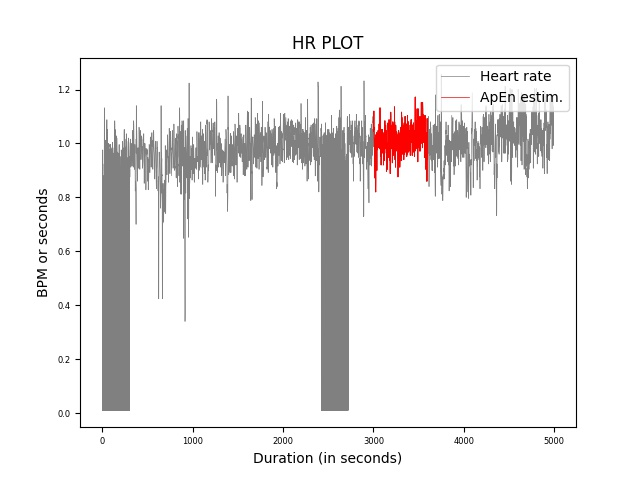
\includegraphics[width=.24\textwidth]{fantasia-Apen/2/fantasia-database-1.0.0_15_f2y10_300sec .jpeg}\hfill
    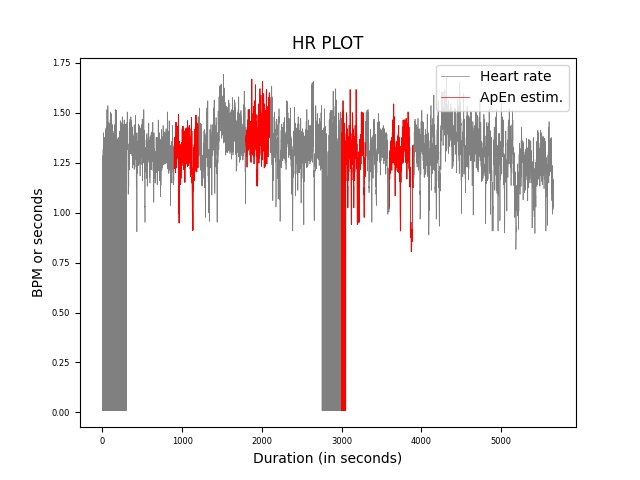
\includegraphics[width=.24\textwidth]{fantasia-Apen/2/fantasia-database-1.0.0_17_f1y04_300sec .jpeg}\hfill
    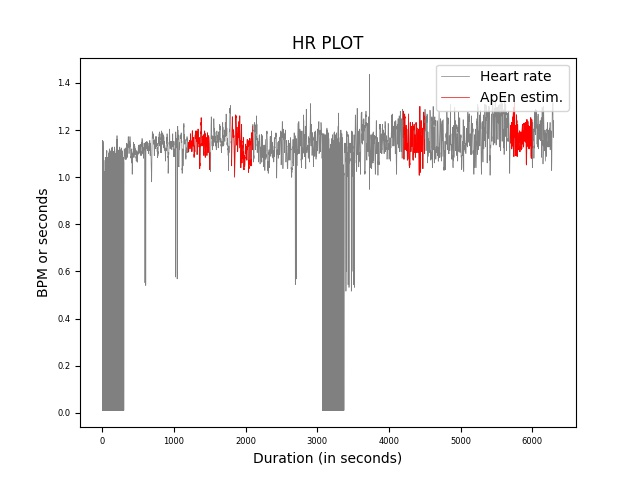
\includegraphics[width=.24\textwidth]{fantasia-Apen/2/fantasia-database-1.0.0_19_f2o09_300sec .jpeg}\hfill
    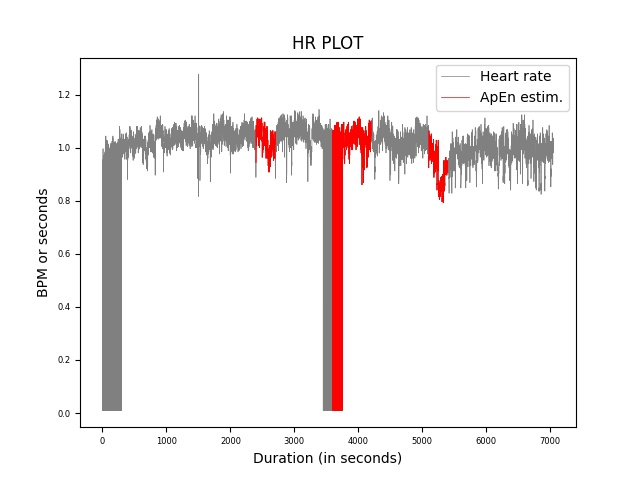
\includegraphics[width=.24\textwidth]{fantasia-Apen/2/fantasia-database-1.0.0_22_f2o04_300sec .jpeg}\hfill
    \\[\smallskipamount]
    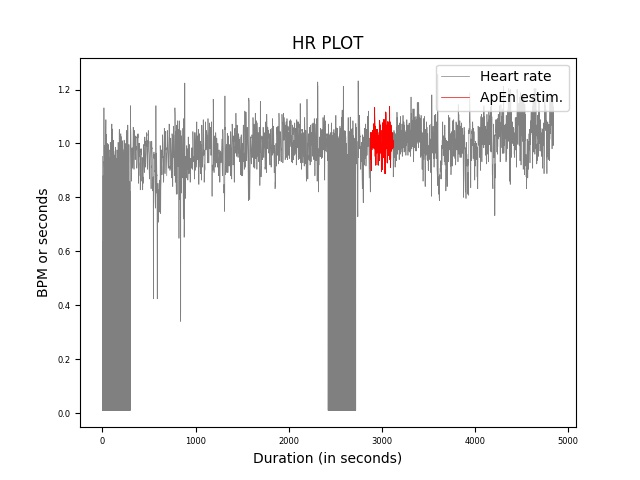
\includegraphics[width=.24\textwidth]{fantasia-Apen/3/fantasia-database-1.0.0_19_f2y10_240sec .jpeg}\hfill
    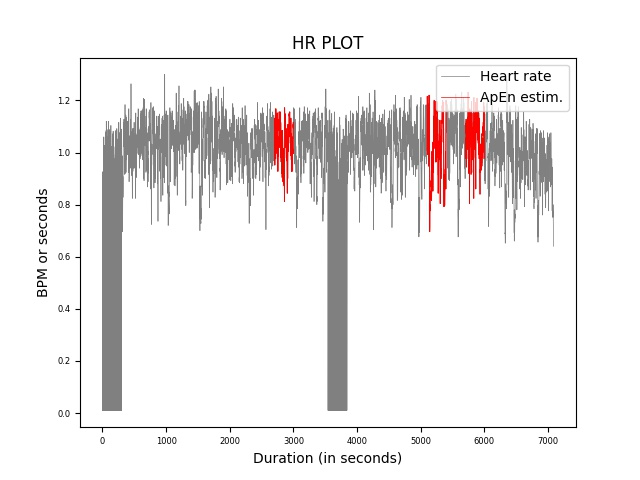
\includegraphics[width=.24\textwidth]{fantasia-Apen/3/fantasia-database-1.0.0_22_f1y06_300sec .jpeg}\hfill
    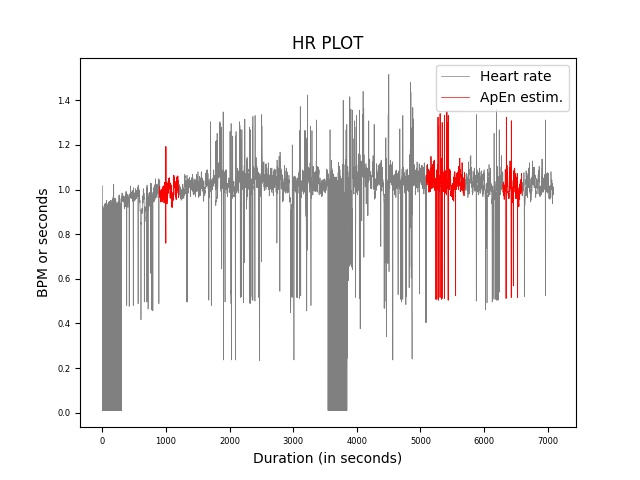
\includegraphics[width=.24\textwidth]{fantasia-Apen/3/fantasia-database-1.0.0_22_f2o08_300sec .jpeg}\hfill
    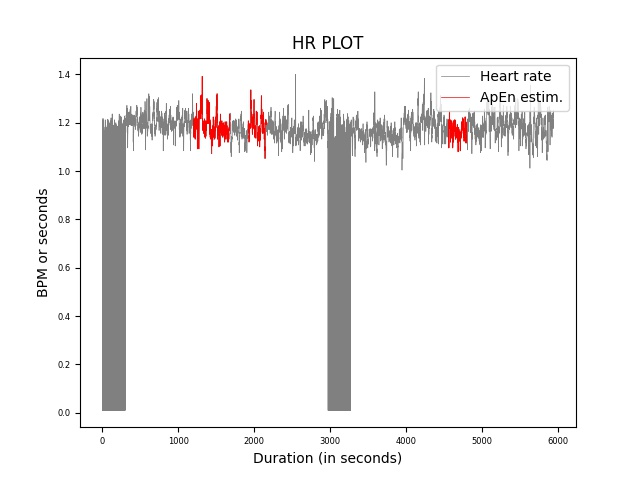
\includegraphics[width=.24\textwidth]{fantasia-Apen/3/fantasia-database-1.0.0_23_f2o07_240sec .jpeg}\hfill
    \\[\smallskipamount]
    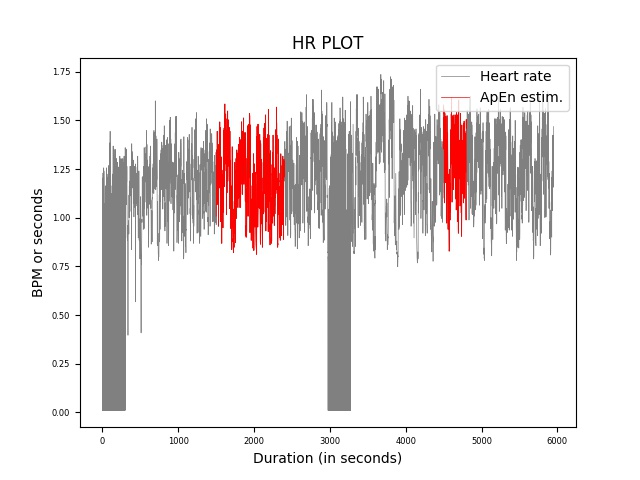
\includegraphics[width=.24\textwidth]{fantasia-Apen/4/fantasia-database-1.0.0_18_f1y07_300sec .jpeg}\hfill
    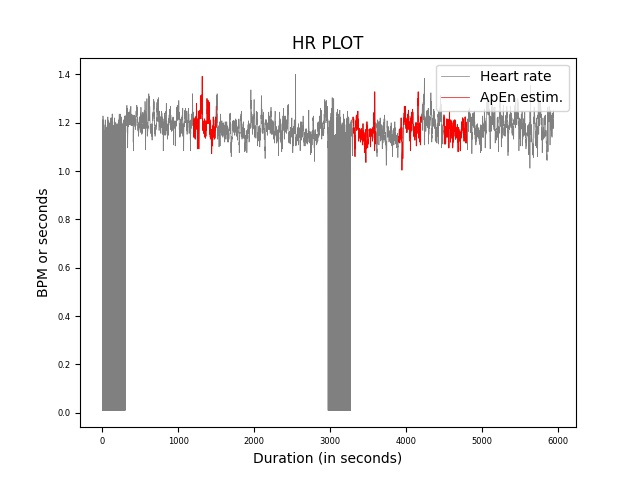
\includegraphics[width=.24\textwidth]{fantasia-Apen/4/fantasia-database-1.0.0_18_f2o07_300sec .jpeg}\hfill
    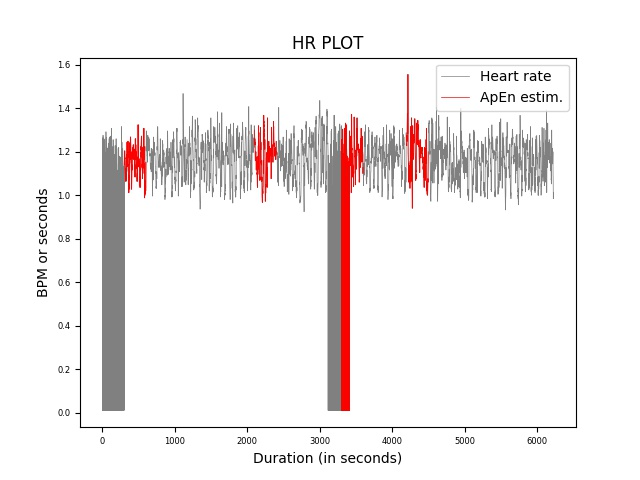
\includegraphics[width=.24\textwidth]{fantasia-Apen/4/fantasia-database-1.0.0_19_f1o04_300sec .jpeg}\hfill
    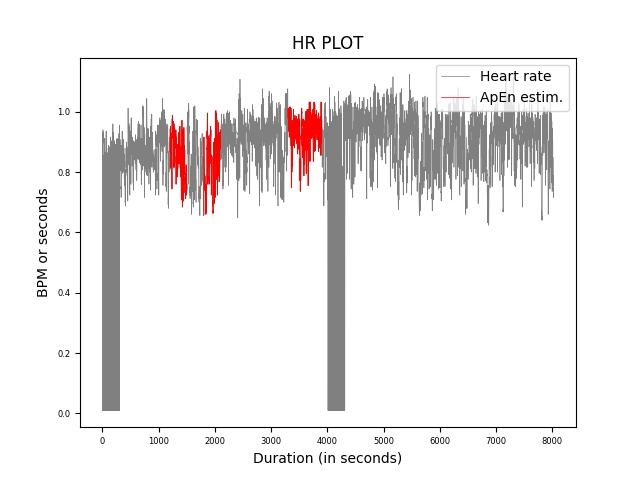
\includegraphics[width=.24\textwidth]{fantasia-Apen/4/fantasia-database-1.0.0_25_f1y09_300sec .jpeg}\hfill
    \\[\smallskipamount]
    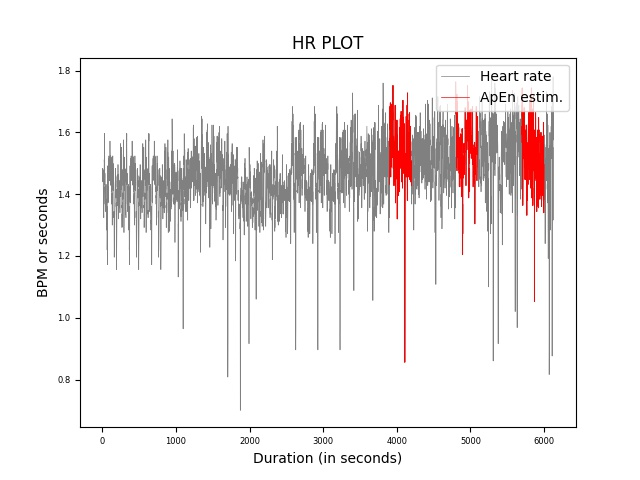
\includegraphics[width=.24\textwidth]{fantasia-Apen/5/fantasia-database-1.0.0_19_f1o09_300sec .jpeg}\hfill
    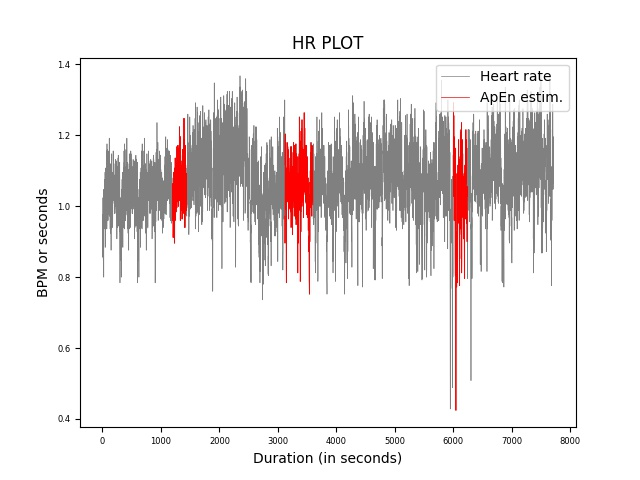
\includegraphics[width=.24\textwidth]{fantasia-Apen/5/fantasia-database-1.0.0_31_f2y07_240sec .jpeg}\hfill
    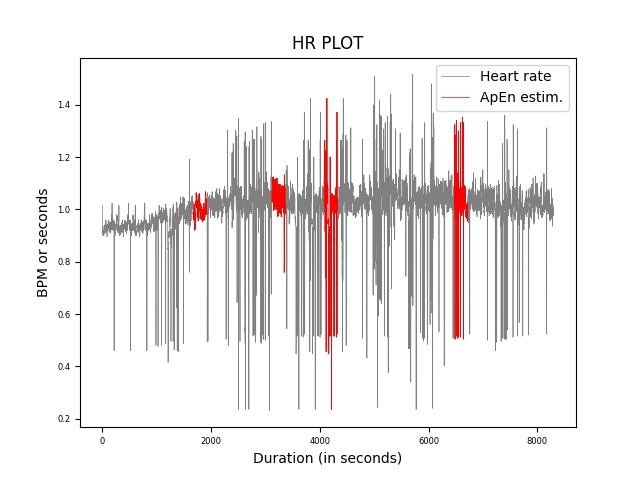
\includegraphics[width=.24\textwidth]{fantasia-Apen/5/fantasia-database-1.0.0_33_f2o08_240sec .jpeg}\hfill
    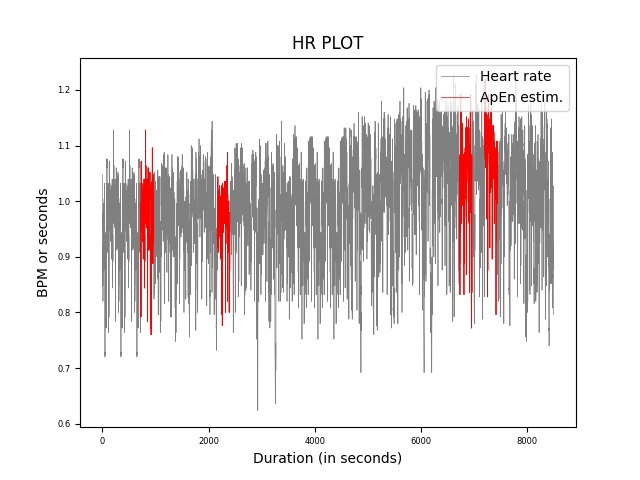
\includegraphics[width=.24\textwidth]{fantasia-Apen/5/fantasia-database-1.0.0_34_f1y08_240sec .jpeg}\hfill
    \\[\smallskipamount]
    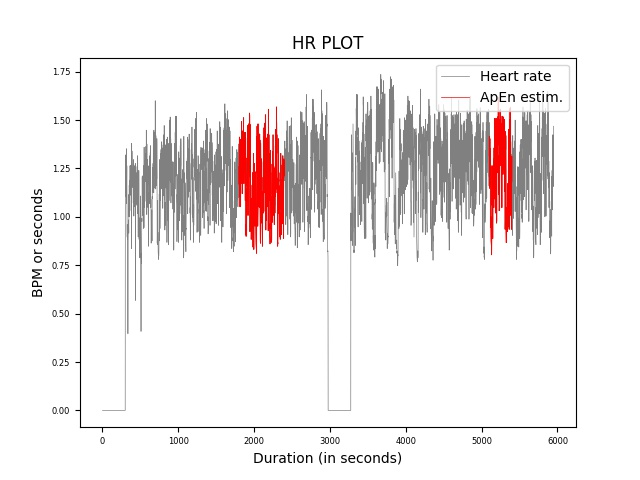
\includegraphics[width=.24\textwidth]{fantasia-Apen/6/fantasia-database-1.0.0_18_f1y07_300sec .jpeg}\hfill
    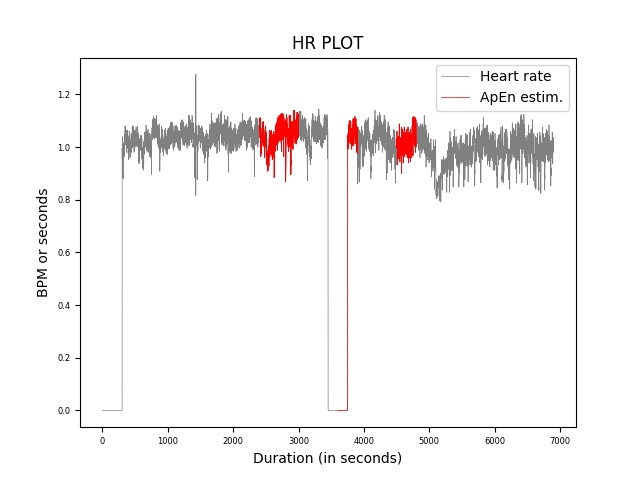
\includegraphics[width=.24\textwidth]{fantasia-Apen/6/fantasia-database-1.0.0_21_f2o04_300sec .jpeg}\hfill
    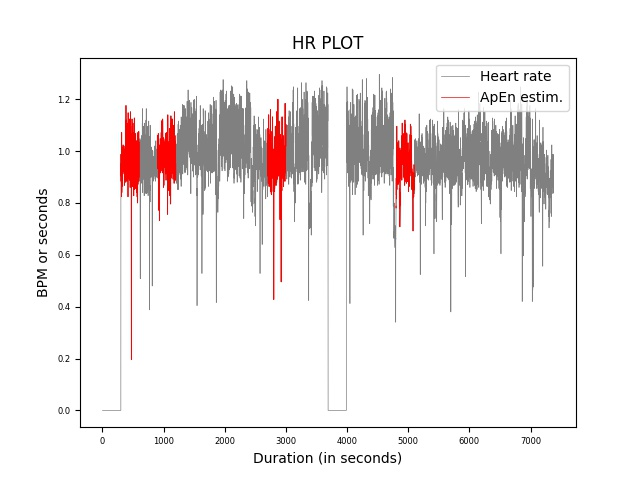
\includegraphics[width=.24\textwidth]{fantasia-Apen/6/fantasia-database-1.0.0_23_f2y08_300sec .jpeg}\hfill
    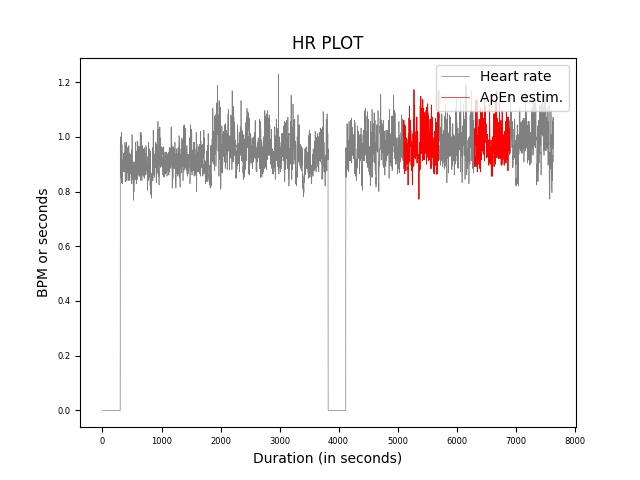
\includegraphics[width=.24\textwidth]{fantasia-Apen/6/fantasia-database-1.0.0_24_f1y03_300sec .jpeg}\hfill
    \caption{Συλλογή αποτελεσμάτων από τη βιβλιοθήκη \en Fantasia Database \gr για τη μετρική \en Apen \gr για τις 6 κατηγορίες πειραμάτων \en AB+C, AxBC, AxB-xC, AxC, \gr πολλαπλασιασμό με τη σταθερά 3 και μηδενισμός συνεχόμενων \en RR \gr διαστημάτων (4 δείγματα από την κάθε κατηγορία)}
\end{figure}

\item \en AVG: \gr Το ίδιο ισχύει για τις υπόλοιπες μετρικές, επομένως και για την \en AVG. \gr Ενώ καταφέρνει να εντοπίσει κάποιες από τις ζητούμενες περιοχές αλλά παραμένει στην κατηγορία των πιο αδύναμων εκτιμήσεων, όπως φαίνεται και στο σχήμα 4.125:

\begin{figure}[h!]
    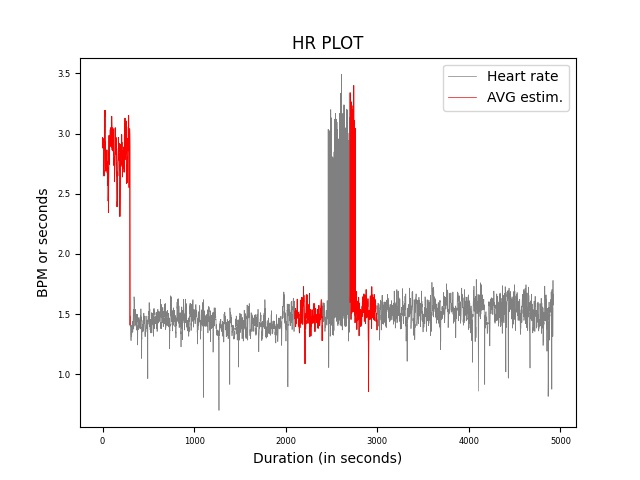
\includegraphics[width=.24\textwidth]{fantasia-AVG/1/fantasia-database-1.0.0_15_f1o09_300sec .jpeg}\hfill
    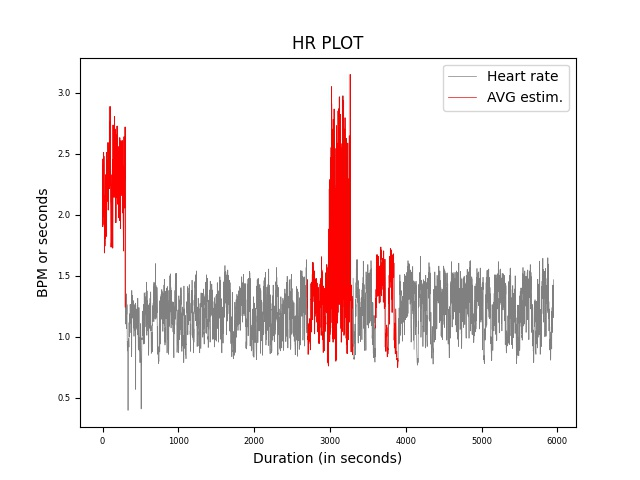
\includegraphics[width=.24\textwidth]{fantasia-AVG/1/fantasia-database-1.0.0_18_f1y07_300sec .jpeg}\hfill
    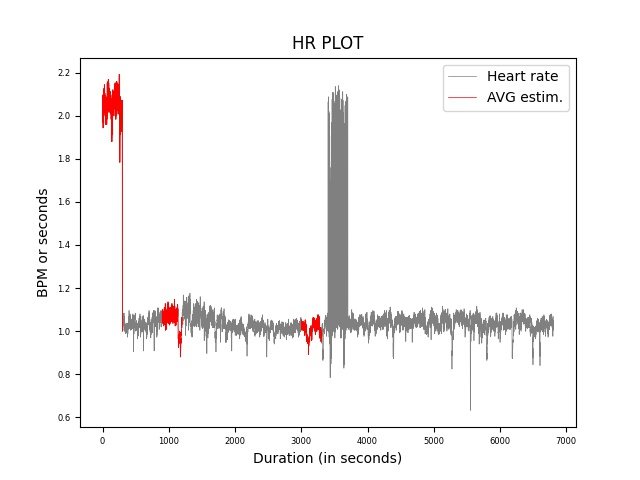
\includegraphics[width=.24\textwidth]{fantasia-AVG/1/fantasia-database-1.0.0_21_f2y03_300sec .jpeg}\hfill
    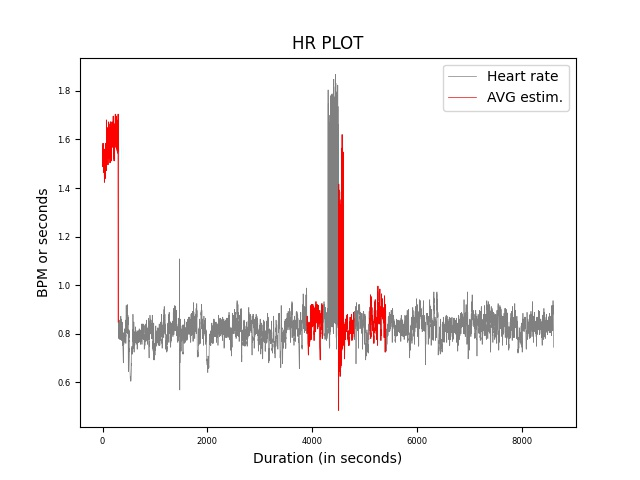
\includegraphics[width=.24\textwidth]{fantasia-AVG/1/fantasia-database-1.0.0_27_f2y04_300sec .jpeg}\hfill
   \\[\smallskipamount]
    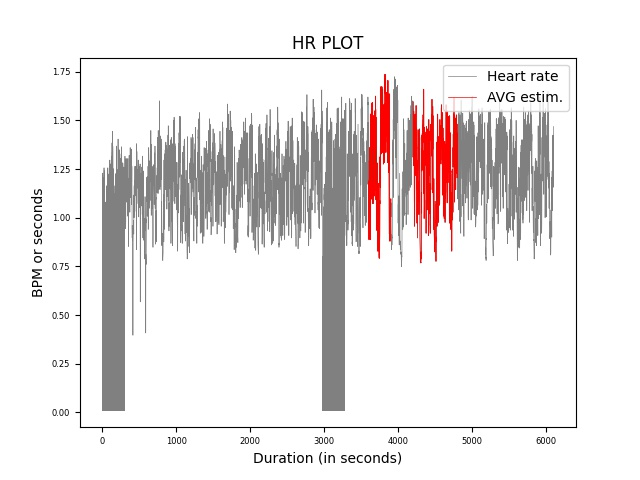
\includegraphics[width=.24\textwidth]{fantasia-AVG/2/fantasia-database-1.0.0_19_f1y07_300sec .jpeg}\hfill
    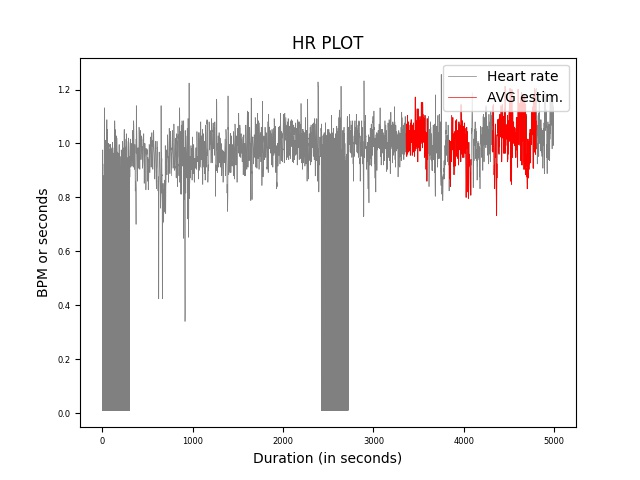
\includegraphics[width=.24\textwidth]{fantasia-AVG/2/fantasia-database-1.0.0_19_f2y10_240sec .jpeg}\hfill
    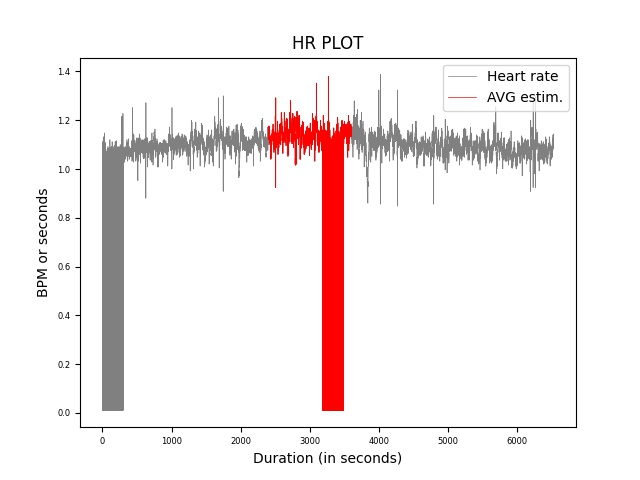
\includegraphics[width=.24\textwidth]{fantasia-AVG/2/fantasia-database-1.0.0_20_f2o02_300sec .jpeg}\hfill
    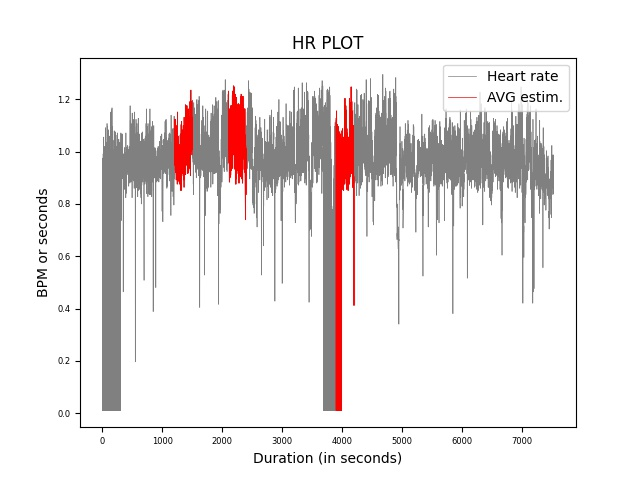
\includegraphics[width=.24\textwidth]{fantasia-AVG/2/fantasia-database-1.0.0_24_f2y08_300sec .jpeg}\hfill
    \\[\smallskipamount]
    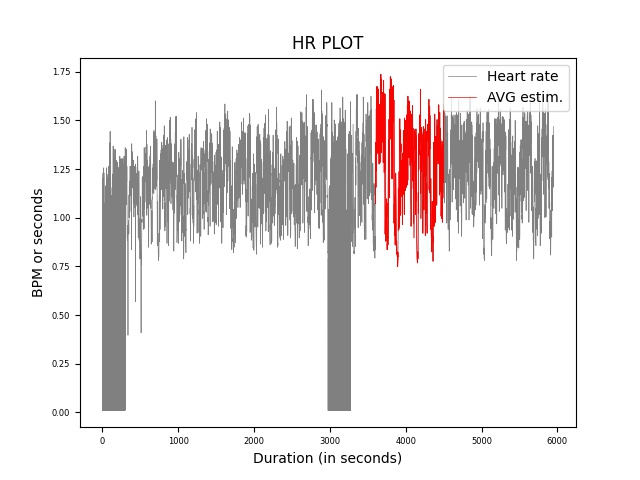
\includegraphics[width=.24\textwidth]{fantasia-AVG/3/fantasia-database-1.0.0_18_f1y07_300sec .jpeg}\hfill
    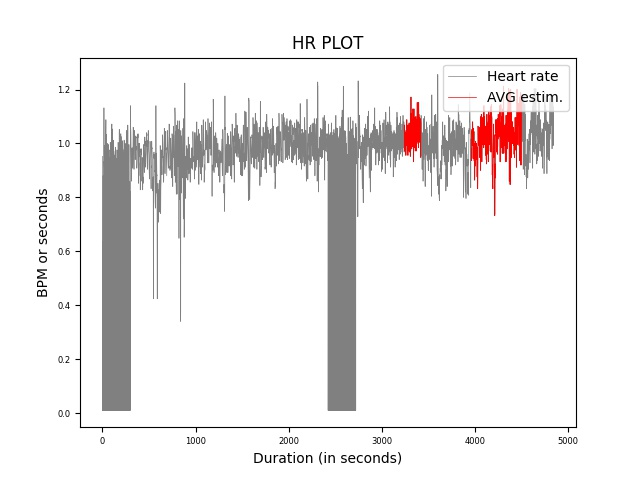
\includegraphics[width=.24\textwidth]{fantasia-AVG/3/fantasia-database-1.0.0_25_f2y10_180sec .jpeg}\hfill
    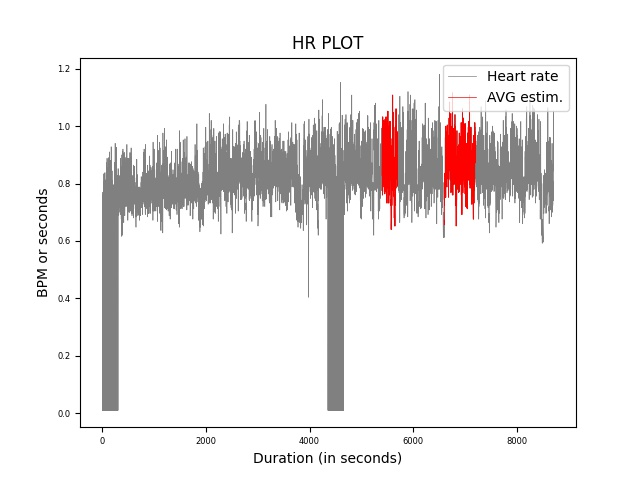
\includegraphics[width=.24\textwidth]{fantasia-AVG/3/fantasia-database-1.0.0_28_f1y01_300sec .jpeg}\hfill
    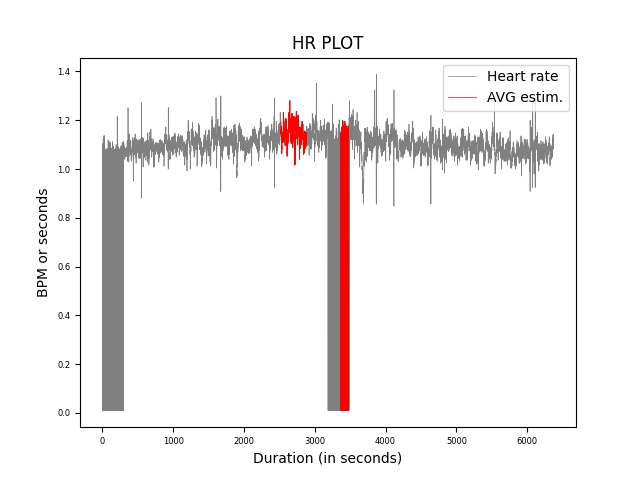
\includegraphics[width=.24\textwidth]{fantasia-AVG/3/fantasia-database-1.0.0_52_f2o02_120sec .jpeg}\hfill
    \\[\smallskipamount]
    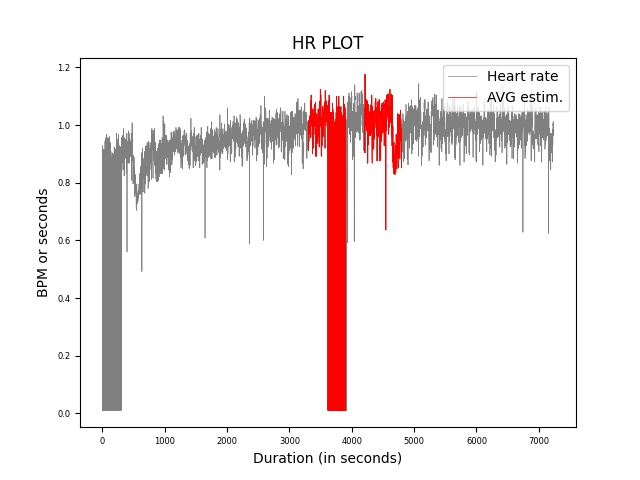
\includegraphics[width=.24\textwidth]{fantasia-AVG/4/fantasia-database-1.0.0_23_f2o01_300sec .jpeg}\hfill
    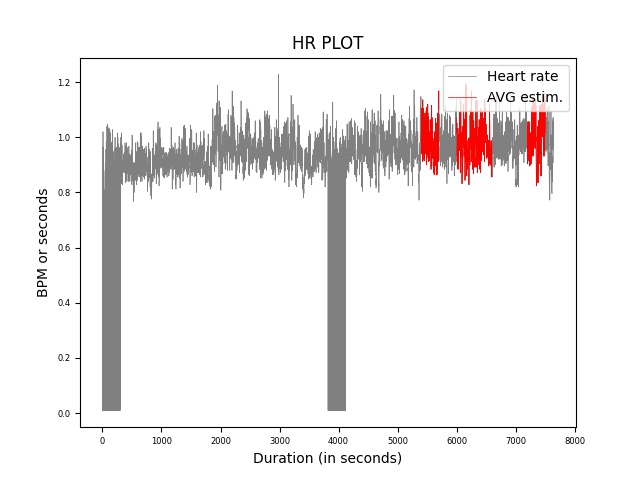
\includegraphics[width=.24\textwidth]{fantasia-AVG/4/fantasia-database-1.0.0_24_f1y03_300sec .jpeg}\hfill
    \includegraphics[width=.24\textwidth]{fantasia-AVG/4/fantasia-database-1.0.0_34_f2o10_240sec .jpeg}\hfill
    \includegraphics[width=.24\textwidth]{fantasia-AVG/4/fantasia-database-1.0.0_39_f2y08_180sec .jpeg}\hfill
    \\[\smallskipamount]
    \includegraphics[width=.24\textwidth]{fantasia-AVG/5/fantasia-database-1.0.0_21_f1y04_300sec .jpeg}\hfill
    \includegraphics[width=.24\textwidth]{fantasia-AVG/5/fantasia-database-1.0.0_25_f2y06_300sec .jpeg}\hfill
    \includegraphics[width=.24\textwidth]{fantasia-AVG/5/fantasia-database-1.0.0_27_f1y08_300sec .jpeg}\hfill
    \includegraphics[width=.24\textwidth]{fantasia-AVG/5/fantasia-database-1.0.0_45_f2o01_180sec .jpeg}\hfill
    \\[\smallskipamount]
    \includegraphics[width=.24\textwidth]{fantasia-AVG/6/fantasia-database-1.0.0_18_f1y07_300sec .jpeg}\hfill
    \includegraphics[width=.24\textwidth]{fantasia-AVG/6/fantasia-database-1.0.0_19_f2y10_240sec .jpeg}\hfill
    \includegraphics[width=.24\textwidth]{fantasia-AVG/6/fantasia-database-1.0.0_20_f2y07_300sec .jpeg}\hfill
    \includegraphics[width=.24\textwidth]{fantasia-AVG/6/fantasia-database-1.0.0_21_f1o02_300sec .jpeg}\hfill
    \caption{Συλλογή αποτελεσμάτων από τη βιβλιοθήκη \en Fantasia Database \gr για τη μετρική \en AVG \gr για τις 6 κατηγορίες πειραμάτων \en AB+C, AxBC, AxB-xC, AxC, \gr πολλαπλασιασμό με τη σταθερά 3 και μηδενισμός συνεχόμενων \en RR \gr διαστημάτων (4 δείγματα από την κάθε κατηγορία)}
\end{figure}

\item \en Bubble: \gr Για τη συγκεκριμένη μέθοδο, οι εκτιμήσεις της ήταν αρκετά έγκυρες στις περιπτώσεις μεταβολής των αρρυθμιών, στη σειρά πειραμάτων με τον τριπλασιασμό των παλμών και το μηδενισμό συνεχόμενων \en RR \gr διαστημάτων, οι εκτιμήσεις δεν ήταν τόσο εύστοχες (Σχήμα 4.126).

\begin{figure}[h!]
    \includegraphics[width=.24\textwidth]{fantasia-Bubble/1/fantasia-database-1.0.0_17_f1y04_300sec .jpeg}\hfill
    \includegraphics[width=.24\textwidth]{fantasia-Bubble/1/fantasia-database-1.0.0_18_f1y07_300sec .jpeg}\hfill
    \includegraphics[width=.24\textwidth]{fantasia-Bubble/1/fantasia-database-1.0.0_18_f2o07_300sec .jpeg}\hfill
    \includegraphics[width=.24\textwidth]{fantasia-Bubble/1/fantasia-database-1.0.0_22_f1o07_300sec .jpeg}\hfill
   \\[\smallskipamount]
    \includegraphics[width=.24\textwidth]{fantasia-Bubble/2/fantasia-database-1.0.0_15_f1o09_300sec .jpeg}\hfill
    \includegraphics[width=.24\textwidth]{fantasia-Bubble/2/fantasia-database-1.0.0_18_f1o05_300sec .jpeg}\hfill
    \includegraphics[width=.24\textwidth]{fantasia-Bubble/2/fantasia-database-1.0.0_19_f1y07_300sec .jpeg}\hfill
    \includegraphics[width=.24\textwidth]{fantasia-Bubble/2/fantasia-database-1.0.0_20_f1o06_300sec .jpeg}\hfill
    \\[\smallskipamount]
    \includegraphics[width=.24\textwidth]{fantasia-Bubble/3/fantasia-database-1.0.0_15_f1o09_300sec .jpeg}\hfill
    \includegraphics[width=.24\textwidth]{fantasia-Bubble/3/fantasia-database-1.0.0_17_f1y04_300sec .jpeg}\hfill
    \includegraphics[width=.24\textwidth]{fantasia-Bubble/3/fantasia-database-1.0.0_18_f1y07_300sec .jpeg}\hfill
    \includegraphics[width=.24\textwidth]{fantasia-Bubble/3/fantasia-database-1.0.0_21_f1o02_300sec .jpeg}\hfill
    \\[\smallskipamount]
    \includegraphics[width=.24\textwidth]{fantasia-Bubble/4/fantasia-database-1.0.0_15_f1o09_300sec .jpeg}\hfill
    \includegraphics[width=.24\textwidth]{fantasia-Bubble/4/fantasia-database-1.0.0_18_f1y07_300sec .jpeg}\hfill
    \includegraphics[width=.24\textwidth]{fantasia-Bubble/4/fantasia-database-1.0.0_22_f1y05_300sec .jpeg}\hfill
    \includegraphics[width=.24\textwidth]{fantasia-Bubble/4/fantasia-database-1.0.0_28_f1y02_240sec .jpeg}\hfill
    \\[\smallskipamount]
    \includegraphics[width=.24\textwidth]{fantasia-Bubble/5/fantasia-database-1.0.0_21_f1y04_300sec .jpeg}\hfill
    \includegraphics[width=.24\textwidth]{fantasia-Bubble/5/fantasia-database-1.0.0_26_f1y06_300sec .jpeg}\hfill
    \includegraphics[width=.24\textwidth]{fantasia-Bubble/5/fantasia-database-1.0.0_29_f1y09_300sec .jpeg}\hfill
    \includegraphics[width=.24\textwidth]{fantasia-Bubble/5/fantasia-database-1.0.0_33_f1y06_240sec .jpeg}\hfill
    \\[\smallskipamount]
    \includegraphics[width=.24\textwidth]{fantasia-Bubble/6/fantasia-database-1.0.0_15_f2y10_300sec .jpeg}\hfill
    \includegraphics[width=.24\textwidth]{fantasia-Bubble/6/fantasia-database-1.0.0_18_f1y07_300sec .jpeg}\hfill
    \includegraphics[width=.24\textwidth]{fantasia-Bubble/6/fantasia-database-1.0.0_20_f2o06_240sec .jpeg}\hfill
    \includegraphics[width=.24\textwidth]{fantasia-Bubble/6/fantasia-database-1.0.0_20_f2y02_300sec .jpeg}\hfill
    \caption{Συλλογή αποτελεσμάτων από τη βιβλιοθήκη \en Fantasia Database \gr για τη μετρική \en Bubble \gr για τις 6 κατηγορίες πειραμάτων \en AB+C, AxBC, AxB-xC, AxC, \gr πολλαπλασιασμό με τη σταθερά 3 και μηδενισμός συνεχόμενων \en RR \gr διαστημάτων (4 δείγματα από την κάθε κατηγορία)}
\end{figure}

\item \en Rényi: \gr Η απόδοσή της διαφέρει ανάλογα με το είδος του πειράματος. Στα πειράματα του μηδενισμού συνεχόμενων τμημάτων, \en AxBC, AxB-xC, AxC \gr τα αποτελέσματα είναι αρκετά επιτυχή, ειδικότερα στα μεγαλύτερα μεγέθη παραθύρου, σε αρκετές περιπτώσεις μάλιστα εντοπίζει όλα τεχνητά τμήματα σε όλα τα δείγματα. Στο πείραμα \en AB+C \gr δεν καταφέρνει να εντοπίσει κανένα από τε τεχνητά τμήματα και εντοπίζει μόνο παλμούς με χαμηλές τιμές (σε αντίθεση με το πείραμα το οποίο δημιουργεί υψηλές τιμές) (Σχήμα 4.127)

\begin{figure}[h!]
    \includegraphics[width=.24\textwidth]{Renyi-fantasia/AB+C/fantasia-database-1.0.0_23_f2o07_240sec .jpeg}\hfill
    \includegraphics[width=.24\textwidth]{Renyi-fantasia/AB+C/fantasia-database-1.0.0_28_f2o08_240sec .jpeg}\hfill
    \includegraphics[width=.24\textwidth]{Renyi-fantasia/AB+C/fantasia-database-1.0.0_30_f1o05_180sec .jpeg}\hfill
    \includegraphics[width=.24\textwidth]{Renyi-fantasia/AB+C/fantasia-database-1.0.0_34_f2o05_240sec .jpeg}\hfill
   \\[\smallskipamount]
    \includegraphics[width=.24\textwidth]{Renyi-fantasia/AxBC/fantasia-database-1.0.0_18_f1o05_300sec .jpeg}\hfill
    \includegraphics[width=.24\textwidth]{Renyi-fantasia/AxBC/fantasia-database-1.0.0_23_f1y06_300sec .jpeg}\hfill
    \includegraphics[width=.24\textwidth]{Renyi-fantasia/AxBC/fantasia-database-1.0.0_23_f1y08_300sec .jpeg}\hfill
    \includegraphics[width=.24\textwidth]{Renyi-fantasia/AxBC/fantasia-database-1.0.0_28_f2y04_300sec .jpeg}\hfill
    \\[\smallskipamount]
    \includegraphics[width=.24\textwidth]{Renyi-fantasia/AxB-xC/fantasia-database-1.0.0_142_f2y04_60sec .jpeg}\hfill
    \includegraphics[width=.24\textwidth]{Renyi-fantasia/AxB-xC/fantasia-database-1.0.0_15_f1o09_300sec .jpeg}\hfill
    \includegraphics[width=.24\textwidth]{Renyi-fantasia/AxB-xC/fantasia-database-1.0.0_22_f1o01_300sec .jpeg}\hfill
    \includegraphics[width=.24\textwidth]{Renyi-fantasia/AxB-xC/fantasia-database-1.0.0_35_f2y07_180sec .jpeg}\hfill
    \\[\smallskipamount]
    \includegraphics[width=.24\textwidth]{Renyi-fantasia/AxC/fantasia-database-1.0.0_36_f1o02_180sec .jpeg}\hfill
    \includegraphics[width=.24\textwidth]{Renyi-fantasia/AxC/fantasia-database-1.0.0_15_f1o09_300sec .jpeg}\hfill
    \includegraphics[width=.24\textwidth]{Renyi-fantasia/AxC/fantasia-database-1.0.0_27_f2o04_240sec .jpeg}\hfill
    \includegraphics[width=.24\textwidth]{Renyi-fantasia/AxC/fantasia-database-1.0.0_29_f1y04_180sec .jpeg}\hfill
    \\[\smallskipamount]
    %\includegraphics[width=.24\textwidth]{}\hfill
    %\includegraphics[width=.24\textwidth]{}\hfill
    %\includegraphics[width=.24\textwidth]{}\hfill
    %\includegraphics[width=.24\textwidth]{}\hfill
    \\[\smallskipamount]
    \includegraphics[width=.24\textwidth]{Renyi-fantasia/zeros/fantasia-database-1.0.0_19_f1o06_300sec .jpeg}\hfill
    \includegraphics[width=.24\textwidth]{Renyi-fantasia/zeros/fantasia-database-1.0.0_20_f2o03_300sec .jpeg}\hfill
    \includegraphics[width=.24\textwidth]{Renyi-fantasia/zeros/fantasia-database-1.0.0_26_f2o03_240sec .jpeg}\hfill
    \includegraphics[width=.24\textwidth]{Renyi-fantasia/zeros/fantasia-database-1.0.0_38_f1o07_180sec .jpeg}\hfill
    \caption{Συλλογή αποτελεσμάτων από τη βιβλιοθήκη \en Fantasia Database \gr για τη μετρική \en Rényi \gr για τις 6 κατηγορίες πειραμάτων \en AB+C, AxBC, AxB-xC, AxC, \gr πολλαπλασιασμό με τη σταθερά 3 και μηδενισμός συνεχόμενων \en RR \gr διαστημάτων (4 δείγματα από την κάθε κατηγορία)}
\end{figure}

\item \en RMSSD: \gr Στο Σχήμα 98 φαίνεται ξεκάθαρα η μεγάλη ευστοχία της μετρικής \en RMSSD. \gr Σε κάθε ένα από τα δείγματα καταφέρνει να εντοπίσει τουλάχιστον τη μία από τις δύο τεχνητές περιοχές στις οποίες το σήμα έχει υποστεί επεξεργασία, αποδίδοντας ξανά ένα από τα καλύτερα αποτελέσματα (Σχήμα 4.128). 

\begin{figure}[h!]
    \includegraphics[width=.24\textwidth]{fantasia-RMSSD/1/fantasia-database-1.0.0_15_f1o09_300sec .jpeg}\hfill
    \includegraphics[width=.24\textwidth]{fantasia-RMSSD/1/fantasia-database-1.0.0_15_f2y10_300sec .jpeg}\hfill
    \includegraphics[width=.24\textwidth]{fantasia-RMSSD/1/fantasia-database-1.0.0_18_f2o07_300sec .jpeg}\hfill
    \includegraphics[width=.24\textwidth]{fantasia-RMSSD/1/fantasia-database-1.0.0_26_f2o03_240sec .jpeg}\hfill
   \\[\smallskipamount]
    \includegraphics[width=.24\textwidth]{fantasia-RMSSD/2/fantasia-database-1.0.0_15_f2y10_300sec .jpeg}\hfill
    \includegraphics[width=.24\textwidth]{fantasia-RMSSD/2/fantasia-database-1.0.0_20_f1o04_300sec .jpeg}\hfill
    \includegraphics[width=.24\textwidth]{fantasia-RMSSD/2/fantasia-database-1.0.0_21_f2o03_300sec .jpeg}\hfill
    \includegraphics[width=.24\textwidth]{fantasia-RMSSD/2/fantasia-database-1.0.0_27_f2y02_240sec .jpeg}\hfill
    \\[\smallskipamount]
    \includegraphics[width=.24\textwidth]{fantasia-RMSSD/3/fantasia-database-1.0.0_118_f1o01_60sec .jpeg}\hfill
    \includegraphics[width=.24\textwidth]{fantasia-RMSSD/3/fantasia-database-1.0.0_140_f2o05_60sec .jpeg}\hfill
    \includegraphics[width=.24\textwidth]{fantasia-RMSSD/3/fantasia-database-1.0.0_23_f1o03_300sec .jpeg}\hfill
    \includegraphics[width=.24\textwidth]{fantasia-RMSSD/3/fantasia-database-1.0.0_76_f2y05_120sec .jpeg}\hfill
    \\[\smallskipamount]
    \includegraphics[width=.24\textwidth]{fantasia-RMSSD/4/fantasia-database-1.0.0_15_f2y10_300sec .jpeg}\hfill
    \includegraphics[width=.24\textwidth]{fantasia-RMSSD/4/fantasia-database-1.0.0_19_f2y10_240sec .jpeg}\hfill
    \includegraphics[width=.24\textwidth]{fantasia-RMSSD/4/fantasia-database-1.0.0_29_f1y04_180sec .jpeg}\hfill
    \includegraphics[width=.24\textwidth]{fantasia-RMSSD/4/fantasia-database-1.0.0_29_f1y08_240sec .jpeg}\hfill
    \\[\smallskipamount]
    \includegraphics[width=.24\textwidth]{fantasia-RMSSD/5/fantasia-database-1.0.0_19_f1o09_300sec .jpeg}\hfill
    \includegraphics[width=.24\textwidth]{fantasia-RMSSD/5/fantasia-database-1.0.0_24_f2y02_300sec .jpeg}\hfill
    \includegraphics[width=.24\textwidth]{fantasia-RMSSD/5/fantasia-database-1.0.0_34_f2o01_240sec .jpeg}\hfill
    \includegraphics[width=.24\textwidth]{fantasia-RMSSD/5/fantasia-database-1.0.0_40_f2y09_240sec .jpeg}\hfill
    \\[\smallskipamount]
    \includegraphics[width=.24\textwidth]{fantasia-RMSSD/6/fantasia-database-1.0.0_15_f1o09_300sec .jpeg}\hfill
    \includegraphics[width=.24\textwidth]{fantasia-RMSSD/6/fantasia-database-1.0.0_21_f1o02_300sec .jpeg}\hfill
    \includegraphics[width=.24\textwidth]{fantasia-RMSSD/6/fantasia-database-1.0.0_21_f1y04_240sec .jpeg}\hfill
    \includegraphics[width=.24\textwidth]{fantasia-RMSSD/6/fantasia-database-1.0.0_65_f1y09_120sec .jpeg}\hfill
    \caption{Συλλογή αποτελεσμάτων από τη βιβλιοθήκη \en Fantasia Database \gr για τη μετρική \en RMSSD \gr για τις 6 κατηγορίες πειραμάτων \en AB+C, AxBC, AxB-xC, AxC, \gr πολλαπλασιασμό με τη σταθερά 3 και μηδενισμός συνεχόμενων \en RR \gr διαστημάτων (4 δείγματα από την κάθε κατηγορία)}
\end{figure}

\item \en SampEn: \gr Για ακόμη μια φορά, η μέθοδος αυτή δεν επιτυγχάνει το επιθυμητό ποσοστό ευστοχίας στις καταγραφές, κάτι που ισχύει στο σύνολο των τεχνητών παλμών και έκτοπων περιοχών. Οι εκτιμήσεις είναι εύκολα αναγνώσιμες στο Σχήμα 99:

\begin{figure}[h!]
    \includegraphics[width=.24\textwidth]{fantasia-SampEn/1/fantasia-database-1.0.0_15_f1o09_300sec .jpeg}\hfill
    \includegraphics[width=.24\textwidth]{fantasia-SampEn/1/fantasia-database-1.0.0_18_f1y07_300sec .jpeg}\hfill
    \includegraphics[width=.24\textwidth]{fantasia-SampEn/1/fantasia-database-1.0.0_23_f1o03_300sec .jpeg}\hfill
    \includegraphics[width=.24\textwidth]{fantasia-SampEn/1/fantasia-database-1.0.0_26_f2y01_300sec .jpeg}\hfill
   \\[\smallskipamount]
    \includegraphics[width=.24\textwidth]{fantasia-SampEn/2/fantasia-database-1.0.0_15_f1o09_300sec .jpeg}\hfill
    \includegraphics[width=.24\textwidth]{fantasia-SampEn/2/fantasia-database-1.0.0_19_f1y07_300sec .jpeg}\hfill
    \includegraphics[width=.24\textwidth]{fantasia-SampEn/2/fantasia-database-1.0.0_20_f1o04_300sec .jpeg}\hfill
    \includegraphics[width=.24\textwidth]{fantasia-SampEn/2/fantasia-database-1.0.0_23_f1o07_300sec .jpeg}\hfill
    \\[\smallskipamount]
    \includegraphics[width=.24\textwidth]{fantasia-SampEn/3/fantasia-database-1.0.0_15_f1o09_300sec .jpeg}\hfill
    \includegraphics[width=.24\textwidth]{fantasia-SampEn/3/fantasia-database-1.0.0_18_f1y07_300sec .jpeg}\hfill
    \includegraphics[width=.24\textwidth]{fantasia-SampEn/3/fantasia-database-1.0.0_20_f2o06_240sec .jpeg}\hfill
    \includegraphics[width=.24\textwidth]{fantasia-SampEn/3/fantasia-database-1.0.0_22_f2o08_300sec .jpeg}\hfill
    \\[\smallskipamount]
    \includegraphics[width=.24\textwidth]{fantasia-SampEn/4/fantasia-database-1.0.0_15_f1o09_300sec .jpeg}\hfill
    \includegraphics[width=.24\textwidth]{fantasia-SampEn/4/fantasia-database-1.0.0_18_f1o05_300sec .jpeg}\hfill
    \includegraphics[width=.24\textwidth]{fantasia-SampEn/4/fantasia-database-1.0.0_18_f1y07_300sec .jpeg}\hfill
    \includegraphics[width=.24\textwidth]{fantasia-SampEn/4/fantasia-database-1.0.0_20_f2o06_240sec .jpeg}\hfill
    \\[\smallskipamount]
    \includegraphics[width=.24\textwidth]{fantasia-SampEn/5/fantasia-database-1.0.0_19_f1o09_300sec .jpeg}\hfill
    \includegraphics[width=.24\textwidth]{fantasia-SampEn/5/fantasia-database-1.0.0_20_f2o06_300sec .jpeg}\hfill
    \includegraphics[width=.24\textwidth]{fantasia-SampEn/5/fantasia-database-1.0.0_22_f1o05_300sec .jpeg}\hfill
    \includegraphics[width=.24\textwidth]{fantasia-SampEn/5/fantasia-database-1.0.0_22_f1y07_300sec .jpeg}\hfill
    \\[\smallskipamount]
    \includegraphics[width=.24\textwidth]{fantasia-SampEn/6/fantasia-database-1.0.0_16_f2o06_300sec .jpeg}\hfill
    \includegraphics[width=.24\textwidth]{fantasia-SampEn/6/fantasia-database-1.0.0_19_f1o09_240sec .jpeg}\hfill
    \includegraphics[width=.24\textwidth]{fantasia-SampEn/6/fantasia-database-1.0.0_20_f2y02_300sec .jpeg}\hfill
    \includegraphics[width=.24\textwidth]{fantasia-SampEn/6/fantasia-database-1.0.0_26_f2y01_300sec .jpeg}\hfill
    \caption{Συλλογή αποτελεσμάτων από τη βιβλιοθήκη \en Fantasia Database \gr για τη μετρική \en SampEn \gr για τις 6 κατηγορίες πειραμάτων \en AB+C, AxBC, AxB-xC, AxC, \gr πολλαπλασιασμό με τη σταθερά 3 και μηδενισμός συνεχόμενων \en RR \gr διαστημάτων (4 δείγματα από την κάθε κατηγορία)}
\end{figure}

\item \en Shannon: \gr Επαναλαμβανόμενα, η μετρική αυτή αποδίδει μέτρια αποτελέσματα αλλά παρόλα αυτά καταφέρνει να εντοπίσει σε κάποιες περιπτώσεις τα ζητούμενα δεδομένα (Σχήμα 100).

\begin{figure}[h!]
    \includegraphics[width=.24\textwidth]{fantasia-Shannon/1/fantasia-database-1.0.0_20_f2y02_300sec .jpeg}\hfill
    \includegraphics[width=.24\textwidth]{fantasia-Shannon/1/fantasia-database-1.0.0_21_f1o02_300sec .jpeg}\hfill
    \includegraphics[width=.24\textwidth]{fantasia-Shannon/1/fantasia-database-1.0.0_21_f1y04_240sec .jpeg}\hfill
    \includegraphics[width=.24\textwidth]{fantasia-Shannon/1/fantasia-database-1.0.0_22_f2o08_300sec .jpeg}\hfill
   \\[\smallskipamount]
    \includegraphics[width=.24\textwidth]{fantasia-Shannon/2/fantasia-database-1.0.0_15_f1o09_300sec .jpeg}\hfill
    \includegraphics[width=.24\textwidth]{fantasia-Shannon/2/fantasia-database-1.0.0_19_f1y07_300sec .jpeg}\hfill
    \includegraphics[width=.24\textwidth]{fantasia-Shannon/2/fantasia-database-1.0.0_20_f1o06_300sec .jpeg}\hfill
    \includegraphics[width=.24\textwidth]{fantasia-Shannon/2/fantasia-database-1.0.0_27_f2o10_300sec .jpeg}\hfill
    \\[\smallskipamount]
    \includegraphics[width=.24\textwidth]{fantasia-Shannon/3/fantasia-database-1.0.0_22_f2o08_300sec .jpeg}\hfill
    \includegraphics[width=.24\textwidth]{fantasia-Shannon/3/fantasia-database-1.0.0_38_f1y06_180sec .jpeg}\hfill
    \includegraphics[width=.24\textwidth]{fantasia-Shannon/3/fantasia-database-1.0.0_52_f2o02_120sec .jpeg}\hfill
    \includegraphics[width=.24\textwidth]{fantasia-Shannon/3/fantasia-database-1.0.0_69_f1o08_120sec .jpeg}\hfill
    \\[\smallskipamount]
    \includegraphics[width=.24\textwidth]{fantasia-Shannon/4/fantasia-database-1.0.0_117_f2o08_60sec .jpeg}\hfill
    \includegraphics[width=.24\textwidth]{fantasia-Shannon/4/fantasia-database-1.0.0_18_f2o07_300sec .jpeg}\hfill
    \includegraphics[width=.24\textwidth]{fantasia-Shannon/4/fantasia-database-1.0.0_22_f2o08_300sec .jpeg}\hfill
    \includegraphics[width=.24\textwidth]{fantasia-Shannon/4/fantasia-database-1.0.0_69_f2o10_120sec .jpeg}\hfill
    \\[\smallskipamount]
    \includegraphics[width=.24\textwidth]{fantasia-Shannon/5/fantasia-database-1.0.0_19_f1o09_300sec .jpeg}\hfill
    \includegraphics[width=.24\textwidth]{fantasia-Shannon/5/fantasia-database-1.0.0_21_f1y04_300sec .jpeg}\hfill
    \includegraphics[width=.24\textwidth]{fantasia-Shannon/5/fantasia-database-1.0.0_24_f1o09_240sec .jpeg}\hfill
    \includegraphics[width=.24\textwidth]{fantasia-Shannon/5/fantasia-database-1.0.0_24_f2y07_300sec .jpeg}\hfill
    \\[\smallskipamount]
    \includegraphics[width=.24\textwidth]{fantasia-Shannon/6/fantasia-database-1.0.0_15_f1o09_300sec .jpeg}\hfill
    \includegraphics[width=.24\textwidth]{fantasia-Shannon/6/fantasia-database-1.0.0_18_f1y07_300sec .jpeg}\hfill
    \includegraphics[width=.24\textwidth]{fantasia-Shannon/6/fantasia-database-1.0.0_21_f2o04_300sec .jpeg}\hfill
    \includegraphics[width=.24\textwidth]{fantasia-Shannon/6/fantasia-database-1.0.0_23_f2y08_300sec .jpeg}\hfill
    \caption{Συλλογή αποτελεσμάτων από τη βιβλιοθήκη \en Fantasia Database \gr για τη μετρική \en Shannon \gr για τις 6 κατηγορίες πειραμάτων \en AB+C, AxBC, AxB-xC, AxC, \gr πολλαπλασιασμό με τη σταθερά 3 και μηδενισμός συνεχόμενων \en RR \gr διαστημάτων (4 δείγματα από την κάθε κατηγορία)}
\end{figure}

\item \en STD: \gr Ό,τι έχει ειπωθεί για τα αποτελέσματα της \en RMSSD \gr ισχύει και σε αυτή την περίπτωση. Σε κάθε ένα από τα δείγματα οι εκτιμήσεις καταφέρνουν να εντοπίσουν και τις δύο τεχνητές περιοχές. Στις περιπτώσεις που αυτό δε συμβαίνει, ο αλγόριθμος εντοπίζει τη μία από τις δυο. Και στις δύο περιπτώσεις πάντως η μετρική φέρνει σε πέρας το στόχο της (Σχήμα 101).

\begin{figure}[h!]
    \includegraphics[width=.24\textwidth]{fantasia-STD/1/fantasia-database-1.0.0_119_f2o01_60sec .jpeg}\hfill
    \includegraphics[width=.24\textwidth]{fantasia-STD/1/fantasia-database-1.0.0_18_f2o07_300sec .jpeg}\hfill
    \includegraphics[width=.24\textwidth]{fantasia-STD/1/fantasia-database-1.0.0_27_f2o10_300sec .jpeg}\hfill
    \includegraphics[width=.24\textwidth]{fantasia-STD/1/fantasia-database-1.0.0_55_f1o02_120sec .jpeg}\hfill
   \\[\smallskipamount]
    \includegraphics[width=.24\textwidth]{fantasia-STD/2/fantasia-database-1.0.0_15_f1o09_300sec .jpeg}\hfill
    \includegraphics[width=.24\textwidth]{fantasia-STD/2/fantasia-database-1.0.0_15_f2y10_300sec .jpeg}\hfill
    \includegraphics[width=.24\textwidth]{fantasia-STD/2/fantasia-database-1.0.0_20_f1o04_300sec .jpeg}\hfill
    \includegraphics[width=.24\textwidth]{fantasia-STD/2/fantasia-database-1.0.0_23_f2o08_300sec .jpeg}\hfill
    \\[\smallskipamount]
    \includegraphics[width=.24\textwidth]{fantasia-STD/3/fantasia-database-1.0.0_15_f2y10_300sec .jpeg}\hfill
    \includegraphics[width=.24\textwidth]{fantasia-STD/3/fantasia-database-1.0.0_20_f2o06_240sec .jpeg}\hfill
    \includegraphics[width=.24\textwidth]{fantasia-STD/3/fantasia-database-1.0.0_22_f1y06_300sec .jpeg}\hfill
    \includegraphics[width=.24\textwidth]{fantasia-STD/3/fantasia-database-1.0.0_25_f1y09_300sec .jpeg}\hfill
    \\[\smallskipamount]
    \includegraphics[width=.24\textwidth]{fantasia-STD/4/fantasia-database-1.0.0_27_f2o10_300sec .jpeg}\hfill
    \includegraphics[width=.24\textwidth]{fantasia-STD/4/fantasia-database-1.0.0_34_f2o10_240sec .jpeg}\hfill
    \includegraphics[width=.24\textwidth]{fantasia-STD/4/fantasia-database-1.0.0_38_f2o08_180sec .jpeg}\hfill
    \includegraphics[width=.24\textwidth]{fantasia-STD/4/fantasia-database-1.0.0_39_f1o03_180sec .jpeg}\hfill
    \\[\smallskipamount]
    \includegraphics[width=.24\textwidth]{fantasia-STD/5/fantasia-database-1.0.0_19_f2y10_300sec .jpeg}\hfill
    \includegraphics[width=.24\textwidth]{fantasia-STD/5/fantasia-database-1.0.0_20_f2o06_300sec .jpeg}\hfill
    \includegraphics[width=.24\textwidth]{fantasia-STD/5/fantasia-database-1.0.0_25_f2y06_300sec .jpeg}\hfill
    \includegraphics[width=.24\textwidth]{fantasia-STD/5/fantasia-database-1.0.0_27_f2o01_300sec .jpeg}\hfill
    \\[\smallskipamount]
    \includegraphics[width=.24\textwidth]{fantasia-STD/6/fantasia-database-1.0.0_15_f1o09_300sec .jpeg}\hfill
    \includegraphics[width=.24\textwidth]{fantasia-STD/6/fantasia-database-1.0.0_16_f2o06_300sec .jpeg}\hfill
    \includegraphics[width=.24\textwidth]{fantasia-STD/6/fantasia-database-1.0.0_20_f2y07_300sec .jpeg}\hfill
    \includegraphics[width=.24\textwidth]{fantasia-STD/6/fantasia-database-1.0.0_22_f2o08_300sec .jpeg}\hfill
    \caption{Συλλογή αποτελεσμάτων από τη βιβλιοθήκη \en Fantasia Database \gr για τη μετρική \en STD \gr για τις 6 κατηγορίες πειραμάτων \en AB+C, AxBC, AxB-xC, AxC, \gr πολλαπλασιασμό με τη σταθερά 3 και μηδενισμός συνεχόμενων \en RR \gr διαστημάτων (4 δείγματα από την κάθε κατηγορία)}
\end{figure}

\item \en Haar wavelets: \gr Σε αυτή τη βιβλιοθήκη φαίνεται η κλίμακα εκτίμησης με την ακρίβεια εντοπισμού των τεχνητών αρρυθμιών/ έκτοπων παλμών είναι δύο ανάλογες παράμετροι. Όσο η κλίμακα αυξάνεται τόσο πιο ακριβής είναι και η απόδοση του αλγορίθμου. Τα αποτελέσματα είναι ορατά στον ακόλουθο πίνακα ο οποίος απεικονίζει την επιτυχία (σε ποσοστιαίο αριθμό, \%) της εκτίμησης των περιοχών ανά κλίμακα κυματιδίων \en Haar \gr σε κάθε μία από τις κατηγορίες πειράματων τεχνητού θορύβου (Πίνακας 1). Παρατηρείται πως δύο συγκεκριμένες κατηγορίες πειραμάτων παρουσιάζουν "ανοσία" στην κλίμακα εκτίμησης των κυματιδίων. Τα πειράματα αυτά είναι ο πολλαπλασιασμός χρονικών διαστημάτων με την αριθμητική σταθερά 3 και το πείραμα \en AB+C \gr και αυτό οφείλεται στη μορφολογία την οποία δημιουργούν στο σήμα. Δημιουργούν υψηλές κορυφές σε ένα κατά τα άλλα φυσιολογικό σήμα, κάτι που κάνει τον εντοπισμό τους ευκολότερο, σε αντίθεση με τις υπολοιπες κατηγορίες. Η ακρίβεια στις εκτιμήσεις του αλγορίθμου φαίνεται να αυξάνεται ραγδαία σε συγκεκριμένες κλίμακες και να παραμένει σχεδόν σταθερή από εκείνο το κατώφλι και μετά. Επομένως, μπορεί να θεωρηθεί πως οι μικρότερες σκάλες εκτίμησης των κυματιδίων δεν αποτελούν κατάλληλες μετρικές (για τις συγκεκριμένες κατηγορίες πειραμάτων).

\begin{table}[h!]
\begin{center}
\caption{{Ποσοστά επιτυχίας με επιτυχία πρόβλεψης τουλάχιστον 50 τοις εκατό (δηλαδή εντοπισμός τουλάχιστον μίας από τις δύο τεχνητές περιοχές) για τη βιβλιοθήκη \en Fantasia Database \gr και όλες τις κλίμακες εκτίμησης των κυματιδίων \en Haar}}
\begin{tabular}{||c | c | c | c | c ||} 
   
 \hline\hline
 \gr Πείραμα & 2 & 3 & 4 & 5   \\ [0.5ex] 
 \hline\hline
\en zeros & 23.68 & 26.31 & 28.94 & 31.57 \\ 
 \hline
\en multiply by 3 & 100 & 100 & 100 & 100 \\
 \hline
\en A B + C & 100 & 100 & 100 & 100 \\
 \hline
\en A x B C & 18.42 & 18.42 & 18.42 & 21.05 \\
 \hline
\en A x B-x C & 26.31 & 39.47 & 26.31 & 23.68 \\ 
 \hline
\en A x C & 26.31 & 36.84 & 31.57 & 23.68 \\ [1ex] 
 \hline
\end{tabular}
\end{center}

\begin{center}
\begin{tabular}{||c | c | c | c | c | c ||} 
   
 \hline\hline
 \gr Πείραμα & 6 & 7 & 8 & 9 & 10  \\ [0.5ex] 
 \hline\hline
\en zeros & 100 & 100 & 100 & 100 & 100 \\ 
 \hline
\en multiply by 3 & 100 & 100 & 100 & 100 & 100 \\
 \hline
\en A B + C & 100 & 100 & 100 & 100 & 88.88 \\
 \hline
\en A x B C & 100 & 100 & 100 & 100 & 100 \\
 \hline
\en A x B-x C & 100 & 97.36 & 100 & 100 & 100 \\ 
 \hline
\en A x C & 100 & 100 & 100 & 100 & 100 \\ [1ex] 
 \hline
\end{tabular}
\end{center}
\end{table}

\end{itemize}
  
 \subsection{\en Normal Sinus Rhythm RR Interval Database \gr}
 Η ίδια διαδικασία ακολουθήθηκε και σε αυτή τη βιβλιοθήκη, μιας και αποτελείται και αυτή από καταγραφές φυσιολογικού σήματος. Για τα κυματίδια \en Haar \gr τα αποτελέσματα είναι ορατά στον Πίνακα 2 για όλες τις σκάλες εκτίμησης και όλες της κατηγορίες πειραμάτων.
\par
Οι παρατηρήσεις για την απόδοση των μετρικών είναι σχεδόν πανομοιότυπα με αυτά της \en Fantasia Database \gr επομένως ο σχολιασμός παραλείπεται προς αποφυγή επαναληψημότητας και εξάντλησης του αναγνώστη.
 \begin{table}[h!]
\begin{center}
\caption{Ποσοστά επιτυχίας με επιτυχία πρόβλεψης τουλάχιστον 50 τοις εκατό (δηλαδή εντοπισμός τουλάχιστον μίας από τις δύο τεχνητές περιοχές) για τη βιβλιοθήκη \en Sinus Rhythm RR Intervals \gr και όλες τις κλίμακες εκτίμησης των κυματιδίων \en Haar}
\begin{tabular}{||c | c | c | c | c ||} 
   
 \hline\hline
 \gr Πείραμα & 2 & 3 & 4 & 5   \\ [0.5ex] 
 \hline\hline
\en zeros & 1.85 & 0 & 1.85 & 79.6 \\ 
 \hline
\en multiply by 3 & 100 & 100 & 100 & 100 \\
 \hline
\en A B + C & 100 & 100 & 100 & 100 \\
 \hline
\en A x B C & 3.7 & 3.7 & 7.4 & 5.55 \\
 \hline
\en A x B-x C & 1.85 & 3.7 & 3.7 & 1.85 \\ 
 \hline
\en A x C & 1.85 & 0 & 5.5 & 1.85 \\ [1ex] 
 \hline
\end{tabular}
\end{center}

\begin{center}
\begin{tabular}{||c | c | c | c | c | c ||} 
   
 \hline\hline
 \gr Πείραμα & 6 & 7 & 8 & 9 & 10  \\ [0.5ex] 
 \hline\hline
\en zeros & 79.62 & 87.03 & 88.88 & 85.18 & 68.51 \\ 
 \hline
\en multiply by 3 & 100 & 100 & 100 & 100 & 100 \\
 \hline
\en A B + C & 100 & 100 & 100 & 100 & 88.88 \\
 \hline
\en A x B C & 88.88 & 90.74 & 94.44 & 88.88 & 88.88 \\
 \hline
\en A x B-x C & 90.74 & 92.59 & 90.74 & 92.59 & 94.44 \\ 
 \hline
\en A x C & 90.74 & 94.44 & 90.74 & 92.59 & 90.74 \\ [1ex] 
 \hline
\end{tabular}

\end{center}
\end{table}

\begin{figure}[h!]
    \includegraphics[width=.24\textwidth]{nsr/normal-sinus-rhythm-rr-interval-database-1.0.0_nsr001.png}\hfill
    \includegraphics[width=.24\textwidth]{nsr/normal-sinus-rhythm-rr-interval-database-1.0.0_nsr004.png}\hfill
    \includegraphics[width=.24\textwidth]{nsr/normal-sinus-rhythm-rr-interval-database-1.0.0_nsr006.png}\hfill
    \includegraphics[width=.24\textwidth]{nsr/normal-sinus-rhythm-rr-interval-database-1.0.0_nsr012.png}\hfill
   \\[\smallskipamount]
    \includegraphics[width=.24\textwidth]{nsr/normal-sinus-rhythm-rr-interval-database-1.0.0_nsr017.png}\hfill
    \includegraphics[width=.24\textwidth]{nsr/normal-sinus-rhythm-rr-interval-database-1.0.0_nsr027.png}\hfill
    \includegraphics[width=.24\textwidth]{nsr/normal-sinus-rhythm-rr-interval-database-1.0.0_nsr029.png}\hfill
    \includegraphics[width=.24\textwidth]{nsr/normal-sinus-rhythm-rr-interval-database-1.0.0_nsr045.png}\hfill
    \\[\smallskipamount]
    \includegraphics[width=.24\textwidth]{nsr/normal-sinus-rhythm-rr-interval-database-1.0.0_nsr048.png}\hfill
    \includegraphics[width=.24\textwidth]{nsr/normal-sinus-rhythm-rr-interval-database-1.0.0_nsr049.png}\hfill
    \includegraphics[width=.24\textwidth]{nsr/normal-sinus-rhythm-rr-interval-database-1.0.0_nsr052.png}\hfill
    \includegraphics[width=.24\textwidth]{nsr/normal-sinus-rhythm-rr-interval-database-1.0.0_nsr053.png}\hfill
    \caption{Συλλογή αποτελεσμάτων από τη βιβλιοθήκη \en Normal Sinus Rhythm RR Interval Database \gr (αρχικά δείγματα/καταγραφές)}
\end{figure}

\begin{figure}[h!]
    \includegraphics[width=.24\textwidth]{nsr-APEn/1/normal-sinus-rhythm-rr-interval-database-1.0.0_341_nsr032_300sec .jpeg}\hfill
    \includegraphics[width=.24\textwidth]{nsr-APEn/1/normal-sinus-rhythm-rr-interval-database-1.0.0_345_nsr043_300sec .jpeg}\hfill
    \includegraphics[width=.24\textwidth]{nsr-APEn/1/normal-sinus-rhythm-rr-interval-database-1.0.0_396_nsr046_240sec .jpeg}\hfill
    \includegraphics[width=.24\textwidth]{nsr-APEn/1/normal-sinus-rhythm-rr-interval-database-1.0.0_599_nsr008_180sec .jpeg}\hfill
   \\[\smallskipamount]
    \includegraphics[width=.24\textwidth]{nsr-APEn/2/normal-sinus-rhythm-rr-interval-database-1.0.0_272_nsr022_300sec .jpeg}\hfill
    \includegraphics[width=.24\textwidth]{nsr-APEn/2/normal-sinus-rhythm-rr-interval-database-1.0.0_549_nsr012_180sec .jpeg}\hfill
    \includegraphics[width=.24\textwidth]{nsr-APEn/2/normal-sinus-rhythm-rr-interval-database-1.0.0_571_nsr006_180sec .jpeg}\hfill
    \includegraphics[width=.24\textwidth]{nsr-APEn/2/normal-sinus-rhythm-rr-interval-database-1.0.0_889_nsr051_120sec .jpeg}\hfill
    \\[\smallskipamount]
    \includegraphics[width=.24\textwidth]{nsr-APEn/3/normal-sinus-rhythm-rr-interval-database-1.0.0_325_nsr004_300sec .jpeg}\hfill
    \includegraphics[width=.24\textwidth]{nsr-APEn/3/normal-sinus-rhythm-rr-interval-database-1.0.0_337_nsr024_300sec .jpeg}\hfill
    \includegraphics[width=.24\textwidth]{nsr-APEn/3/normal-sinus-rhythm-rr-interval-database-1.0.0_339_nsr022_240sec .jpeg}\hfill
    \includegraphics[width=.24\textwidth]{nsr-APEn/3/normal-sinus-rhythm-rr-interval-database-1.0.0_600_nsr028_180sec .jpeg}\hfill
    \\[\smallskipamount]
    \includegraphics[width=.24\textwidth]{nsr-APEn/4/normal-sinus-rhythm-rr-interval-database-1.0.0_559_nsr017_180sec .jpeg}\hfill
    \includegraphics[width=.24\textwidth]{nsr-APEn/4/normal-sinus-rhythm-rr-interval-database-1.0.0_548_nsr012_180sec .jpeg}\hfill
    \includegraphics[width=.24\textwidth]{nsr-APEn/4/normal-sinus-rhythm-rr-interval-database-1.0.0_568_nsr020_240sec .jpeg}\hfill
    \includegraphics[width=.24\textwidth]{nsr-APEn/4/normal-sinus-rhythm-rr-interval-database-1.0.0_875_nsr030_120sec .jpeg}\hfill
    \\[\smallskipamount]
    \includegraphics[width=.24\textwidth]{nsr-APEn/5/normal-sinus-rhythm-rr-interval-database-1.0.0_332_nsr012_300sec .jpeg}\hfill
    \includegraphics[width=.24\textwidth]{nsr-APEn/5/normal-sinus-rhythm-rr-interval-database-1.0.0_343_nsr038_300sec .jpeg}\hfill
    \includegraphics[width=.24\textwidth]{nsr-APEn/5/normal-sinus-rhythm-rr-interval-database-1.0.0_404_nsr016_240sec .jpeg}\hfill
    \includegraphics[width=.24\textwidth]{nsr-APEn/5/normal-sinus-rhythm-rr-interval-database-1.0.0_555_nsr012_180sec .jpeg}\hfill
    \\[\smallskipamount]
    \includegraphics[width=.24\textwidth]{nsr-APEn/6/normal-sinus-rhythm-rr-interval-database-1.0.0_1929_nsr013_60sec .jpeg}\hfill
    \includegraphics[width=.24\textwidth]{nsr-APEn/6/normal-sinus-rhythm-rr-interval-database-1.0.0_372_nsr014_300sec .jpeg}\hfill
    \includegraphics[width=.24\textwidth]{nsr-APEn/6/normal-sinus-rhythm-rr-interval-database-1.0.0_372_nsr023_300sec .jpeg}\hfill
    \includegraphics[width=.24\textwidth]{nsr-APEn/6/normal-sinus-rhythm-rr-interval-database-1.0.0_381_nsr036_300sec .jpeg}\hfill
    \caption{Συλλογή αποτελεσμάτων από τη βιβλιοθήκη \en Normal Sinus Rhythm RR Interval Database \gr για τη μετρική \en ApEn \gr για τις 6 κατηγορίες πειραμάτων \en AB+C, AxBC, AxB-xC, AxC, \gr πολλαπλασιασμό με τη σταθερά 3 και μηδενισμός συνεχόμενων \en RR \gr διαστημάτων (4 δείγματα από την κάθε κατηγορία)}
\end{figure}

\begin{figure}[h!]
    \includegraphics[width=.24\textwidth]{nsr-AVG/1/normal-sinus-rhythm-rr-interval-database-1.0.0_319_nsr016_300sec .jpeg}\hfill
    \includegraphics[width=.24\textwidth]{nsr-AVG/1/normal-sinus-rhythm-rr-interval-database-1.0.0_372_nsr014_300sec .jpeg}\hfill
    \includegraphics[width=.24\textwidth]{nsr-AVG/1/normal-sinus-rhythm-rr-interval-database-1.0.0_465_nsr014_240sec .jpeg}\hfill
    \includegraphics[width=.24\textwidth]{nsr-AVG/1/normal-sinus-rhythm-rr-interval-database-1.0.0_570_nsr009_180sec .jpeg}\hfill
   \\[\smallskipamount]
    \includegraphics[width=.24\textwidth]{nsr-AVG/2/normal-sinus-rhythm-rr-interval-database-1.0.0_272_nsr022_300sec .jpeg}\hfill
    \includegraphics[width=.24\textwidth]{nsr-AVG/2/normal-sinus-rhythm-rr-interval-database-1.0.0_372_nsr014_300sec .jpeg}\hfill
    \includegraphics[width=.24\textwidth]{nsr-AVG/2/normal-sinus-rhythm-rr-interval-database-1.0.0_491_nsr035_240sec .jpeg}\hfill
    \includegraphics[width=.24\textwidth]{nsr-AVG/2/normal-sinus-rhythm-rr-interval-database-1.0.0_511_nsr019_240sec .jpeg}\hfill
    \\[\smallskipamount]
    \includegraphics[width=.24\textwidth]{nsr-AVG/3/normal-sinus-rhythm-rr-interval-database-1.0.0_1702_nsr038_60sec .jpeg}\hfill
    \includegraphics[width=.24\textwidth]{nsr-AVG/3/normal-sinus-rhythm-rr-interval-database-1.0.0_2154_nsr025_60sec .jpeg}\hfill
    \includegraphics[width=.24\textwidth]{nsr-AVG/3/normal-sinus-rhythm-rr-interval-database-1.0.0_337_nsr024_300sec .jpeg}\hfill
    \includegraphics[width=.24\textwidth]{nsr-AVG/3/normal-sinus-rhythm-rr-interval-database-1.0.0_875_nsr030_120sec .jpeg}\hfill
    \\[\smallskipamount]
    \includegraphics[width=.24\textwidth]{nsr-AVG/4/normal-sinus-rhythm-rr-interval-database-1.0.0_339_nsr038_300sec .jpeg}\hfill
    \includegraphics[width=.24\textwidth]{nsr-AVG/4/normal-sinus-rhythm-rr-interval-database-1.0.0_345_nsr021_300sec .jpeg}\hfill
    \includegraphics[width=.24\textwidth]{nsr-AVG/4/normal-sinus-rhythm-rr-interval-database-1.0.0_537_nsr025_240sec .jpeg}\hfill
    \includegraphics[width=.24\textwidth]{nsr-AVG/4/normal-sinus-rhythm-rr-interval-database-1.0.0_757_nsr020_180sec .jpeg}\hfill
    \\[\smallskipamount]
    \includegraphics[width=.24\textwidth]{nsr-AVG/5/normal-sinus-rhythm-rr-interval-database-1.0.0_345_nsr009_300sec .jpeg}\hfill
    \includegraphics[width=.24\textwidth]{nsr-AVG/5/normal-sinus-rhythm-rr-interval-database-1.0.0_363_nsr008_300sec .jpeg}\hfill
    \includegraphics[width=.24\textwidth]{nsr-AVG/5/normal-sinus-rhythm-rr-interval-database-1.0.0_561_nsr039_180sec .jpeg}\hfill
    \includegraphics[width=.24\textwidth]{nsr-AVG/5/normal-sinus-rhythm-rr-interval-database-1.0.0_661_nsr035_180sec .jpeg}\hfill
    \\[\smallskipamount]
    \includegraphics[width=.24\textwidth]{nsr-AVG/6/normal-sinus-rhythm-rr-interval-database-1.0.0_339_nsr038_300sec .jpeg}\hfill
    \includegraphics[width=.24\textwidth]{nsr-AVG/6/normal-sinus-rhythm-rr-interval-database-1.0.0_355_nsr001_300sec .jpeg}\hfill
    \includegraphics[width=.24\textwidth]{nsr-AVG/6/normal-sinus-rhythm-rr-interval-database-1.0.0_487_nsr005_240sec .jpeg}\hfill
    \includegraphics[width=.24\textwidth]{nsr-AVG/6/normal-sinus-rhythm-rr-interval-database-1.0.0_801_nsr010_120sec .jpeg}\hfill
    \caption{Συλλογή αποτελεσμάτων από τη βιβλιοθήκη \en Normal Sinus Rhythm RR Interval Database \gr για τη μετρική \en AVG \gr για τις 6 κατηγορίες πειραμάτων \en AB+C, AxBC, AxB-xC, AxC, \gr πολλαπλασιασμό με τη σταθερά 3 και μηδενισμός συνεχόμενων \en RR \gr διαστημάτων (4 δείγματα από την κάθε κατηγορία)}
\end{figure}

\begin{figure}[h!]
    \includegraphics[width=.24\textwidth]{nsr-Bubble/1/normal-sinus-rhythm-rr-interval-database-1.0.0_372_nsr014_300sec .jpeg}\hfill
    \includegraphics[width=.24\textwidth]{nsr-Bubble/1/normal-sinus-rhythm-rr-interval-database-1.0.0_408_nsr019_300sec .jpeg}\hfill
    \includegraphics[width=.24\textwidth]{nsr-Bubble/1/normal-sinus-rhythm-rr-interval-database-1.0.0_485_nsr026_240sec .jpeg}\hfill
    \includegraphics[width=.24\textwidth]{nsr-Bubble/1/normal-sinus-rhythm-rr-interval-database-1.0.0_864_nsr021_120sec .jpeg}\hfill
   \\[\smallskipamount]
    \includegraphics[width=.24\textwidth]{nsr-Bubble/2/normal-sinus-rhythm-rr-interval-database-1.0.0_256_nsr033_300sec .jpeg}\hfill
    \includegraphics[width=.24\textwidth]{nsr-Bubble/2/normal-sinus-rhythm-rr-interval-database-1.0.0_326_nsr034_300sec .jpeg}\hfill
    \includegraphics[width=.24\textwidth]{nsr-Bubble/2/normal-sinus-rhythm-rr-interval-database-1.0.0_400_nsr016_240sec .jpeg}\hfill
    \includegraphics[width=.24\textwidth]{nsr-Bubble/2/normal-sinus-rhythm-rr-interval-database-1.0.0_428_nsr006_240sec .jpeg}\hfill
    \\[\smallskipamount]
    \includegraphics[width=.24\textwidth]{nsr-Bubble/3/normal-sinus-rhythm-rr-interval-database-1.0.0_1855_nsr002_60sec .jpeg}\hfill
    \includegraphics[width=.24\textwidth]{nsr-Bubble/3/normal-sinus-rhythm-rr-interval-database-1.0.0_1867_nsr023_60sec .jpeg}\hfill
    \includegraphics[width=.24\textwidth]{nsr-Bubble/3/normal-sinus-rhythm-rr-interval-database-1.0.0_1966_nsr035_60sec .jpeg}\hfill
    \includegraphics[width=.24\textwidth]{nsr-Bubble/3/normal-sinus-rhythm-rr-interval-database-1.0.0_466_nsr023_240sec .jpeg}\hfill
    \\[\smallskipamount]
    \includegraphics[width=.24\textwidth]{nsr-Bubble/4/normal-sinus-rhythm-rr-interval-database-1.0.0_332_nsr039_300sec .jpeg}\hfill
    \includegraphics[width=.24\textwidth]{nsr-Bubble/4/normal-sinus-rhythm-rr-interval-database-1.0.0_335_nsr017_300sec .jpeg}\hfill
    \includegraphics[width=.24\textwidth]{nsr-Bubble/4/normal-sinus-rhythm-rr-interval-database-1.0.0_339_nsr022_240sec .jpeg}\hfill
    \includegraphics[width=.24\textwidth]{nsr-Bubble/4/normal-sinus-rhythm-rr-interval-database-1.0.0_424_nsr015_240sec .jpeg}\hfill
    \\[\smallskipamount]
    \includegraphics[width=.24\textwidth]{nsr-Bubble/5/normal-sinus-rhythm-rr-interval-database-1.0.0_325_nsr033_240sec .jpeg}\hfill
    \includegraphics[width=.24\textwidth]{nsr-Bubble/5/normal-sinus-rhythm-rr-interval-database-1.0.0_343_nsr038_300sec .jpeg}\hfill
    \includegraphics[width=.24\textwidth]{nsr-Bubble/5/normal-sinus-rhythm-rr-interval-database-1.0.0_360_nsr007_300sec .jpeg}\hfill
    \includegraphics[width=.24\textwidth]{nsr-Bubble/5/normal-sinus-rhythm-rr-interval-database-1.0.0_385_nsr036_300sec .jpeg}\hfill
    \\[\smallskipamount]
    \includegraphics[width=.24\textwidth]{nsr-Bubble/6/normal-sinus-rhythm-rr-interval-database-1.0.0_332_nsr039_300sec .jpeg}\hfill
    \includegraphics[width=.24\textwidth]{nsr-Bubble/6/normal-sinus-rhythm-rr-interval-database-1.0.0_400_nsr010_240sec .jpeg}\hfill
    \includegraphics[width=.24\textwidth]{nsr-Bubble/6/normal-sinus-rhythm-rr-interval-database-1.0.0_415_nsr039_240sec .jpeg}\hfill
    \includegraphics[width=.24\textwidth]{nsr-Bubble/6/normal-sinus-rhythm-rr-interval-database-1.0.0_424_nsr038_240sec .jpeg}\hfill
    \caption{Συλλογή αποτελεσμάτων από τη βιβλιοθήκη \en Normal Sinus Rhythm RR Interval Database \gr για τη μετρική \en Bubble \gr για τις 6 κατηγορίες πειραμάτων \en AB+C, AxBC, AxB-xC, AxC, \gr πολλαπλασιασμό με τη σταθερά 3 και μηδενισμός συνεχόμενων \en RR \gr διαστημάτων (4 δείγματα από την κάθε κατηγορία)}
\end{figure}

\begin{figure}[h!]
    \includegraphics[width=.24\textwidth]{nsr-Bubble/1/normal-sinus-rhythm-rr-interval-database-1.0.0_372_nsr014_300sec .jpeg}\hfill
    \includegraphics[width=.24\textwidth]{nsr-Bubble/1/normal-sinus-rhythm-rr-interval-database-1.0.0_408_nsr019_300sec .jpeg}\hfill
    \includegraphics[width=.24\textwidth]{nsr-Bubble/1/normal-sinus-rhythm-rr-interval-database-1.0.0_485_nsr026_240sec .jpeg}\hfill
    \includegraphics[width=.24\textwidth]{nsr-Bubble/1/normal-sinus-rhythm-rr-interval-database-1.0.0_864_nsr021_120sec .jpeg}\hfill
   \\[\smallskipamount]
    \includegraphics[width=.24\textwidth]{nsr-Bubble/2/normal-sinus-rhythm-rr-interval-database-1.0.0_256_nsr033_300sec .jpeg}\hfill
    \includegraphics[width=.24\textwidth]{nsr-Bubble/2/normal-sinus-rhythm-rr-interval-database-1.0.0_326_nsr034_300sec .jpeg}\hfill
    \includegraphics[width=.24\textwidth]{nsr-Bubble/2/normal-sinus-rhythm-rr-interval-database-1.0.0_400_nsr016_240sec .jpeg}\hfill
    \includegraphics[width=.24\textwidth]{nsr-Bubble/2/normal-sinus-rhythm-rr-interval-database-1.0.0_428_nsr006_240sec .jpeg}\hfill
    \\[\smallskipamount]
    \includegraphics[width=.24\textwidth]{nsr-Bubble/3/normal-sinus-rhythm-rr-interval-database-1.0.0_1855_nsr002_60sec .jpeg}\hfill
    \includegraphics[width=.24\textwidth]{nsr-Bubble/3/normal-sinus-rhythm-rr-interval-database-1.0.0_1867_nsr023_60sec .jpeg}\hfill
    \includegraphics[width=.24\textwidth]{nsr-Bubble/3/normal-sinus-rhythm-rr-interval-database-1.0.0_1966_nsr035_60sec .jpeg}\hfill
    \includegraphics[width=.24\textwidth]{nsr-Bubble/3/normal-sinus-rhythm-rr-interval-database-1.0.0_466_nsr023_240sec .jpeg}\hfill
    \\[\smallskipamount]
    \includegraphics[width=.24\textwidth]{nsr-Bubble/4/normal-sinus-rhythm-rr-interval-database-1.0.0_332_nsr039_300sec .jpeg}\hfill
    \includegraphics[width=.24\textwidth]{nsr-Bubble/4/normal-sinus-rhythm-rr-interval-database-1.0.0_335_nsr017_300sec .jpeg}\hfill
    \includegraphics[width=.24\textwidth]{nsr-Bubble/4/normal-sinus-rhythm-rr-interval-database-1.0.0_339_nsr022_240sec .jpeg}\hfill
    \includegraphics[width=.24\textwidth]{nsr-Bubble/4/normal-sinus-rhythm-rr-interval-database-1.0.0_424_nsr015_240sec .jpeg}\hfill
    \\[\smallskipamount]
    \includegraphics[width=.24\textwidth]{nsr-Bubble/5/normal-sinus-rhythm-rr-interval-database-1.0.0_325_nsr033_240sec .jpeg}\hfill
    \includegraphics[width=.24\textwidth]{nsr-Bubble/5/normal-sinus-rhythm-rr-interval-database-1.0.0_343_nsr038_300sec .jpeg}\hfill
    \includegraphics[width=.24\textwidth]{nsr-Bubble/5/normal-sinus-rhythm-rr-interval-database-1.0.0_360_nsr007_300sec .jpeg}\hfill
    \includegraphics[width=.24\textwidth]{nsr-Bubble/5/normal-sinus-rhythm-rr-interval-database-1.0.0_385_nsr036_300sec .jpeg}\hfill
    \\[\smallskipamount]
    \includegraphics[width=.24\textwidth]{nsr-Bubble/6/normal-sinus-rhythm-rr-interval-database-1.0.0_332_nsr039_300sec .jpeg}\hfill
    \includegraphics[width=.24\textwidth]{nsr-Bubble/6/normal-sinus-rhythm-rr-interval-database-1.0.0_400_nsr010_240sec .jpeg}\hfill
    \includegraphics[width=.24\textwidth]{nsr-Bubble/6/normal-sinus-rhythm-rr-interval-database-1.0.0_415_nsr039_240sec .jpeg}\hfill
    \includegraphics[width=.24\textwidth]{nsr-Bubble/6/normal-sinus-rhythm-rr-interval-database-1.0.0_424_nsr038_240sec .jpeg}\hfill
    \caption{Συλλογή αποτελεσμάτων από τη βιβλιοθήκη \en Normal Sinus Rhythm RR Interval Database \gr για τη μετρική \en Rényi \gr για τις 6 κατηγορίες πειραμάτων \en AB+C, AxBC, AxB-xC, AxC, \gr πολλαπλασιασμό με τη σταθερά 3 και μηδενισμός συνεχόμενων \en RR \gr διαστημάτων (4 δείγματα από την κάθε κατηγορία)}
\end{figure}

\begin{figure}[h!]
    \includegraphics[width=.24\textwidth]{Renyi-nsr/AB+C/normal-sinus-rhythm-rr-interval-database-1.0.0_1944_nsr026_60sec .jpeg}\hfill
    \includegraphics[width=.24\textwidth]{Renyi-nsr/AB+C/normal-sinus-rhythm-rr-interval-database-1.0.0_348_nsr049_300sec .jpeg}\hfill
    \includegraphics[width=.24\textwidth]{Renyi-nsr/AB+C/normal-sinus-rhythm-rr-interval-database-1.0.0_354_nsr051_300sec .jpeg}\hfill
    \includegraphics[width=.24\textwidth]{Renyi-nsr/AB+C/normal-sinus-rhythm-rr-interval-database-1.0.0_566_nsr038_180sec .jpeg}\hfill
   \\[\smallskipamount]
   \includegraphics[width=.24\textwidth]{Renyi-nsr/AxBC/normal-sinus-rhythm-rr-interval-database-1.0.0_256_nsr033_300sec .jpeg}\hfill
    \includegraphics[width=.24\textwidth]{Renyi-nsr/AxBC/normal-sinus-rhythm-rr-interval-database-1.0.0_272_nsr022_300sec .jpeg}\hfill
    \includegraphics[width=.24\textwidth]{Renyi-nsr/AxBC/normal-sinus-rhythm-rr-interval-database-1.0.0_349_nsr049_300sec .jpeg}\hfill
    \includegraphics[width=.24\textwidth]{Renyi-nsr/AxBC/normal-sinus-rhythm-rr-interval-database-1.0.0_389_nsr037_240sec .jpeg}\hfill
    \\[\smallskipamount]
    \includegraphics[width=.24\textwidth]{Renyi-nsr/AxB-xC/normal-sinus-rhythm-rr-interval-database-1.0.0_271_nsr022_300sec .jpeg}\hfill
    \includegraphics[width=.24\textwidth]{Renyi-nsr/AxB-xC/normal-sinus-rhythm-rr-interval-database-1.0.0_342_nsr041_300sec .jpeg}\hfill
    \includegraphics[width=.24\textwidth]{Renyi-nsr/AxB-xC/normal-sinus-rhythm-rr-interval-database-1.0.0_359_nsr008_300sec .jpeg}\hfill
    \includegraphics[width=.24\textwidth]{Renyi-nsr/AxB-xC/normal-sinus-rhythm-rr-interval-database-1.0.0_390_nsr048_300sec .jpeg}\hfill
    \\[\smallskipamount]    
    %\includegraphics[width=.24\textwidth]{}\hfill
    %\includegraphics[width=.24\textwidth]{nsr-RMSSD/4/normal-sinus-rhythm-rr-interval-database-1.0.0_2275_nsr020_60sec .jpeg}\hfill
    %\includegraphics[width=.24\textwidth]{nsr-RMSSD/4/normal-sinus-rhythm-rr-interval-database-1.0.0_621_nsr023_180sec .jpeg}\hfill
    %\includegraphics[width=.24\textwidth]{nsr-RMSSD/4/normal-sinus-rhythm-rr-interval-database-1.0.0_641_nsr033_120sec .jpeg}\hfill
    \\[\smallskipamount]
    \includegraphics[width=.24\textwidth]{Renyi-nsr/multiply/normal-sinus-rhythm-rr-interval-database-1.0.0_325_nsr004_300sec .jpeg}\hfill
    \includegraphics[width=.24\textwidth]{Renyi-nsr/multiply/normal-sinus-rhythm-rr-interval-database-1.0.0_339_nsr015_300sec .jpeg}\hfill
    \includegraphics[width=.24\textwidth]{Renyi-nsr/multiply/normal-sinus-rhythm-rr-interval-database-1.0.0_388_nsr026_300sec .jpeg}\hfill
    \includegraphics[width=.24\textwidth]{Renyi-nsr/multiply/normal-sinus-rhythm-rr-interval-database-1.0.0_399_nsr016_240sec .jpeg}\hfill
    \\[\smallskipamount]
    %\includegraphics[width=.24\textwidth]{nsr-RMSSD/6/normal-sinus-rhythm-rr-interval-database-1.0.0_645_nsr011_180sec .jpeg}\hfill
    %\includegraphics[width=.24\textwidth]{nsr-RMSSD/6/normal-sinus-rhythm-rr-interval-database-1.0.0_654_nsr035_180sec .jpeg}\hfill
    %\includegraphics[width=.24\textwidth]{nsr-RMSSD/6/normal-sinus-rhythm-rr-interval-database-1.0.0_927_nsr002_120sec .jpeg}\hfill
    %\includegraphics[width=.24\textwidth]{nsr-RMSSD/6/normal-sinus-rhythm-rr-interval-database-1.0.0_964_nsr013_120sec .jpeg}\hfill
    \caption{Συλλογή αποτελεσμάτων από τη βιβλιοθήκη \en Normal Sinus Rhythm RR Interval Database \gr για τη μετρική \en RMSSD \gr για τις 6 κατηγορίες πειραμάτων \en AB+C, AxBC, AxB-xC, AxC, \gr πολλαπλασιασμό με τη σταθερά 3 και μηδενισμός συνεχόμενων \en RR \gr διαστημάτων (4 δείγματα από την κάθε κατηγορία)}
\end{figure}

\begin{figure}[h!]
    \includegraphics[width=.24\textwidth]{nsr-SampEn/1/normal-sinus-rhythm-rr-interval-database-1.0.0_1557_nsr037_60sec .jpeg}\hfill
    \includegraphics[width=.24\textwidth]{nsr-SampEn/1/normal-sinus-rhythm-rr-interval-database-1.0.0_1867_nsr023_60sec .jpeg}\hfill
    \includegraphics[width=.24\textwidth]{nsr-SampEn/1/normal-sinus-rhythm-rr-interval-database-1.0.0_372_nsr014_300sec .jpeg}\hfill
    \includegraphics[width=.24\textwidth]{nsr-SampEn/1/normal-sinus-rhythm-rr-interval-database-1.0.0_431_nsr021_240sec .jpeg}\hfill
   \\[\smallskipamount]
    \includegraphics[width=.24\textwidth]{nsr-SampEn/2/normal-sinus-rhythm-rr-interval-database-1.0.0_1078_nsr025_120sec .jpeg}\hfill
    \includegraphics[width=.24\textwidth]{nsr-SampEn/2/normal-sinus-rhythm-rr-interval-database-1.0.0_2049_nsr019_60sec .jpeg}\hfill
    \includegraphics[width=.24\textwidth]{nsr-SampEn/2/normal-sinus-rhythm-rr-interval-database-1.0.0_567_nsr038_180sec .jpeg}\hfill
    \includegraphics[width=.24\textwidth]{nsr-SampEn/2/normal-sinus-rhythm-rr-interval-database-1.0.0_571_nsr006_180sec .jpeg}\hfill
    \\[\smallskipamount]
    \includegraphics[width=.24\textwidth]{nsr-SampEn/3/normal-sinus-rhythm-rr-interval-database-1.0.0_1953_nsr005_60sec .jpeg}\hfill
    \includegraphics[width=.24\textwidth]{nsr-SampEn/3/normal-sinus-rhythm-rr-interval-database-1.0.0_2275_nsr020_60sec .jpeg}\hfill
    \includegraphics[width=.24\textwidth]{nsr-SampEn/3/normal-sinus-rhythm-rr-interval-database-1.0.0_592_nsr001_180sec .jpeg}\hfill
    \includegraphics[width=.24\textwidth]{nsr-SampEn/3/normal-sinus-rhythm-rr-interval-database-1.0.0_889_nsr001_120sec .jpeg}\hfill
    \\[\smallskipamount]
    \includegraphics[width=.24\textwidth]{nsr-SampEn/4/normal-sinus-rhythm-rr-interval-database-1.0.0_355_nsr001_300sec .jpeg}\hfill
    \includegraphics[width=.24\textwidth]{nsr-SampEn/4/normal-sinus-rhythm-rr-interval-database-1.0.0_372_nsr023_300sec .jpeg}\hfill
    \includegraphics[width=.24\textwidth]{nsr-SampEn/4/normal-sinus-rhythm-rr-interval-database-1.0.0_427_nsr006_240sec .jpeg}\hfill
    \includegraphics[width=.24\textwidth]{nsr-SampEn/4/normal-sinus-rhythm-rr-interval-database-1.0.0_431_nsr021_240sec .jpeg}\hfill
    \\[\smallskipamount]
    \includegraphics[width=.24\textwidth]{nsr-SampEn/5/normal-sinus-rhythm-rr-interval-database-1.0.0_1653_nsr034_60sec .jpeg}\hfill
    \includegraphics[width=.24\textwidth]{nsr-SampEn/5/normal-sinus-rhythm-rr-interval-database-1.0.0_2295_nsr020_60sec .jpeg}\hfill
    \includegraphics[width=.24\textwidth]{nsr-SampEn/5/normal-sinus-rhythm-rr-interval-database-1.0.0_573_nsr038_180sec .jpeg}\hfill
    \includegraphics[width=.24\textwidth]{nsr-SampEn/5/normal-sinus-rhythm-rr-interval-database-1.0.0_582_nsr021_180sec .jpeg}\hfill
    \\[\smallskipamount]
    \includegraphics[width=.24\textwidth]{nsr-SampEn/6/normal-sinus-rhythm-rr-interval-database-1.0.0_2275_nsr020_60sec .jpeg}\hfill
    \includegraphics[width=.24\textwidth]{nsr-SampEn/6/normal-sinus-rhythm-rr-interval-database-1.0.0_381_nsr036_300sec .jpeg}\hfill
    \includegraphics[width=.24\textwidth]{nsr-SampEn/6/normal-sinus-rhythm-rr-interval-database-1.0.0_931_nsr014_120sec .jpeg}\hfill
    \includegraphics[width=.24\textwidth]{nsr-SampEn/6/normal-sinus-rhythm-rr-interval-database-1.0.0_933_nsr023_120sec .jpeg}\hfill
    \caption{Συλλογή αποτελεσμάτων από τη βιβλιοθήκη \en Normal Sinus Rhythm RR Interval Database \gr για τη μετρική \en SampEn \gr για τις 6 κατηγορίες πειραμάτων \en AB+C, AxBC, AxB-xC, AxC, \gr πολλαπλασιασμό με τη σταθερά 3 και μηδενισμός συνεχόμενων \en RR \gr διαστημάτων (4 δείγματα από την κάθε κατηγορία)}
\end{figure}

\begin{figure}[h!]
    \includegraphics[width=.24\textwidth]{nsr-Shannon/1/normal-sinus-rhythm-rr-interval-database-1.0.0_271_nsr022_300sec .jpeg}\hfill
    \includegraphics[width=.24\textwidth]{nsr-Shannon/1/normal-sinus-rhythm-rr-interval-database-1.0.0_325_nsr034_300sec .jpeg}\hfill
    \includegraphics[width=.24\textwidth]{nsr-Shannon/1/normal-sinus-rhythm-rr-interval-database-1.0.0_332_nsr039_300sec .jpeg}\hfill
    \includegraphics[width=.24\textwidth]{nsr-Shannon/1/normal-sinus-rhythm-rr-interval-database-1.0.0_342_nsr006_300sec .jpeg}\hfill
   \\[\smallskipamount]
    \includegraphics[width=.24\textwidth]{nsr-Shannon/2/normal-sinus-rhythm-rr-interval-database-1.0.0_1931_nsr013_60sec .jpeg}\hfill
    \includegraphics[width=.24\textwidth]{nsr-Shannon/2/normal-sinus-rhythm-rr-interval-database-1.0.0_2278_nsr020_60sec .jpeg}\hfill
    \includegraphics[width=.24\textwidth]{nsr-Shannon/2/normal-sinus-rhythm-rr-interval-database-1.0.0_487_nsr029_240sec .jpeg}\hfill
    \includegraphics[width=.24\textwidth]{nsr-Shannon/2/normal-sinus-rhythm-rr-interval-database-1.0.0_900_nsr008_120sec .jpeg}\hfill
    \\[\smallskipamount]
    \includegraphics[width=.24\textwidth]{nsr-Shannon/3/normal-sinus-rhythm-rr-interval-database-1.0.0_392_nsr035_300sec .jpeg}\hfill
    \includegraphics[width=.24\textwidth]{nsr-Shannon/3/normal-sinus-rhythm-rr-interval-database-1.0.0_431_nsr021_240sec .jpeg}\hfill
    \includegraphics[width=.24\textwidth]{nsr-Shannon/3/normal-sinus-rhythm-rr-interval-database-1.0.0_444_nsr001_240sec .jpeg}\hfill
    \includegraphics[width=.24\textwidth]{nsr-Shannon/3/normal-sinus-rhythm-rr-interval-database-1.0.0_840_nsr017_120sec .jpeg}\hfill
    \\[\smallskipamount]
    \includegraphics[width=.24\textwidth]{nsr-Shannon/4/normal-sinus-rhythm-rr-interval-database-1.0.0_319_nsr010_300sec .jpeg}\hfill
    \includegraphics[width=.24\textwidth]{nsr-Shannon/4/normal-sinus-rhythm-rr-interval-database-1.0.0_372_nsr014_300sec .jpeg}\hfill
    \includegraphics[width=.24\textwidth]{nsr-Shannon/4/normal-sinus-rhythm-rr-interval-database-1.0.0_388_nsr037_240sec .jpeg}\hfill
    \includegraphics[width=.24\textwidth]{nsr-Shannon/4/normal-sinus-rhythm-rr-interval-database-1.0.0_389_nsr005_300sec .jpeg}\hfill
    \\[\smallskipamount]
    \includegraphics[width=.24\textwidth]{nsr-Shannon/5/normal-sinus-rhythm-rr-interval-database-1.0.0_1653_nsr034_60sec .jpeg}\hfill
    \includegraphics[width=.24\textwidth]{nsr-Shannon/5/normal-sinus-rhythm-rr-interval-database-1.0.0_341_nsr024_300sec .jpeg}\hfill
    \includegraphics[width=.24\textwidth]{nsr-Shannon/5/normal-sinus-rhythm-rr-interval-database-1.0.0_343_nsr038_300sec .jpeg}\hfill
    \includegraphics[width=.24\textwidth]{nsr-Shannon/5/normal-sinus-rhythm-rr-interval-database-1.0.0_456_nsr018_240sec .jpeg}\hfill
    \\[\smallskipamount]
    \includegraphics[width=.24\textwidth]{nsr-Shannon/6/normal-sinus-rhythm-rr-interval-database-1.0.0_1966_nsr035_60sec .jpeg}\hfill
    \includegraphics[width=.24\textwidth]{nsr-Shannon/6/normal-sinus-rhythm-rr-interval-database-1.0.0_392_nsr035_300sec .jpeg}\hfill
    \includegraphics[width=.24\textwidth]{nsr-Shannon/6/normal-sinus-rhythm-rr-interval-database-1.0.0_421_nsr024_240sec .jpeg}\hfill
    \includegraphics[width=.24\textwidth]{nsr-Shannon/6/normal-sinus-rhythm-rr-interval-database-1.0.0_566_nsr038_180sec .jpeg}\hfill
    \caption{Συλλογή αποτελεσμάτων από τη βιβλιοθήκη \en Normal Sinus Rhythm RR Interval Database \gr για τη μετρική \en Shannon \gr για τις 6 κατηγορίες πειραμάτων \en AB+C, AxBC, AxB-xC, AxC, \gr πολλαπλασιασμό με τη σταθερά 3 και μηδενισμός συνεχόμενων \en RR \gr διαστημάτων (4 δείγματα από την κάθε κατηγορία)}
\end{figure}

\begin{figure}[h!]
    \includegraphics[width=.24\textwidth]{nsr-STD/1/normal-sinus-rhythm-rr-interval-database-1.0.0_255_nsr033_300sec .jpeg}\hfill
    \includegraphics[width=.24\textwidth]{nsr-STD/1/normal-sinus-rhythm-rr-interval-database-1.0.0_324_nsr003_300sec .jpeg}\hfill
    \includegraphics[width=.24\textwidth]{nsr-STD/1/normal-sinus-rhythm-rr-interval-database-1.0.0_337_nsr024_300sec .jpeg}\hfill
    \includegraphics[width=.24\textwidth]{nsr-STD/1/normal-sinus-rhythm-rr-interval-database-1.0.0_360_nsr018_300sec .jpeg}\hfill
   \\[\smallskipamount]
    \includegraphics[width=.24\textwidth]{nsr-STD/2/normal-sinus-rhythm-rr-interval-database-1.0.0_256_nsr033_300sec .jpeg}\hfill
    \includegraphics[width=.24\textwidth]{nsr-STD/2/normal-sinus-rhythm-rr-interval-database-1.0.0_682_nsr019_180sec .jpeg}\hfill
    \includegraphics[width=.24\textwidth]{nsr-STD/2/normal-sinus-rhythm-rr-interval-database-1.0.0_965_nsr013_120sec .jpeg}\hfill
    \includegraphics[width=.24\textwidth]{nsr-STD/2/normal-sinus-rhythm-rr-interval-database-1.0.0_977_nsr005_120sec .jpeg}\hfill
    \\[\smallskipamount]
    \includegraphics[width=.24\textwidth]{nsr-STD/3/normal-sinus-rhythm-rr-interval-database-1.0.0_1022_nsr019_120sec .jpeg}\hfill
    \includegraphics[width=.24\textwidth]{nsr-STD/3/normal-sinus-rhythm-rr-interval-database-1.0.0_386_nsr011_300sec .jpeg}\hfill
    \includegraphics[width=.24\textwidth]{nsr-STD/3/normal-sinus-rhythm-rr-interval-database-1.0.0_372_nsr014_300sec .jpeg}\hfill
    \includegraphics[width=.24\textwidth]{nsr-STD/3/normal-sinus-rhythm-rr-interval-database-1.0.0_595_nsr007_180sec .jpeg}\hfill
    \\[\smallskipamount]
    \includegraphics[width=.24\textwidth]{nsr-STD/4/normal-sinus-rhythm-rr-interval-database-1.0.0_381_nsr036_300sec .jpeg}\hfill
    \includegraphics[width=.24\textwidth]{nsr-STD/4/normal-sinus-rhythm-rr-interval-database-1.0.0_388_nsr037_240sec .jpeg}\hfill
    \includegraphics[width=.24\textwidth]{nsr-STD/4/normal-sinus-rhythm-rr-interval-database-1.0.0_626_nsr027_180sec .jpeg}\hfill
    \includegraphics[width=.24\textwidth]{nsr-STD/4/normal-sinus-rhythm-rr-interval-database-1.0.0_850_nsr015_120sec .jpeg}\hfill
    \\[\smallskipamount]
    \includegraphics[width=.24\textwidth]{nsr-STD/5/normal-sinus-rhythm-rr-interval-database-1.0.0_1147_nsr020_120sec .jpeg}\hfill
    \includegraphics[width=.24\textwidth]{nsr-STD/5/normal-sinus-rhythm-rr-interval-database-1.0.0_2295_nsr020_60sec .jpeg}\hfill
    \includegraphics[width=.24\textwidth]{nsr-STD/5/normal-sinus-rhythm-rr-interval-database-1.0.0_569_nsr024_180sec .jpeg}\hfill
    \includegraphics[width=.24\textwidth]{nsr-STD/5/normal-sinus-rhythm-rr-interval-database-1.0.0_577_nsr006_180sec .jpeg}\hfill
    \\[\smallskipamount]
    \includegraphics[width=.24\textwidth]{nsr-STD/6/normal-sinus-rhythm-rr-interval-database-1.0.0_355_nsr001_300sec .jpeg}\hfill
    \includegraphics[width=.24\textwidth]{nsr-STD/6/normal-sinus-rhythm-rr-interval-database-1.0.0_360_nsr018_300sec .jpeg}\hfill
    \includegraphics[width=.24\textwidth]{nsr-STD/6/normal-sinus-rhythm-rr-interval-database-1.0.0_487_nsr029_240sec .jpeg}\hfill
    \includegraphics[width=.24\textwidth]{nsr-STD/6/normal-sinus-rhythm-rr-interval-database-1.0.0_566_nsr038_180sec .jpeg}\hfill
    \caption{Συλλογή αποτελεσμάτων από τη βιβλιοθήκη \en Normal Sinus Rhythm RR Interval Database \gr για τη μετρική \en STD \gr για τις 6 κατηγορίες πειραμάτων \en AB+C, AxBC, AxB-xC, AxC, \gr πολλαπλασιασμό με τη σταθερά 3 και μηδενισμός συνεχόμενων \en RR \gr διαστημάτων (4 δείγματα από την κάθε κατηγορία)}
\end{figure}

%\end{document}